%%%%%%%%%%%%%%%%%%%%%%%%%%%%%%%%%%%%%%%%%
% Beamer Presentation
% LaTeX Template
% Version 2.0 (March 8, 2022)
%
% This template originates from:
% https://www.LaTeXTemplates.com
%
% Author:
% Vel (vel@latextemplates.com)
%
% License:
% CC BY-NC-SA 4.0 (https://creativecommons.org/licenses/by-nc-sa/4.0/)
%
%%%%%%%%%%%%%%%%%%%%%%%%%%%%%%%%%%%%%%%%%

%----------------------------------------------------------------------------------------
%	PACKAGES AND OTHER DOCUMENT CONFIGURATIONS
%----------------------------------------------------------------------------------------

\documentclass[
	11pt, % Set the default font size, options include: 8pt, 9pt, 10pt, 11pt, 12pt, 14pt, 17pt, 20pt
	%t, % Uncomment to vertically align all slide content to the top of the slide, rather than the default centered
	%aspectratio=169, % Uncomment to set the aspect ratio to a 16:9 ratio which matches the aspect ratio of 1080p and 4K screens and projectors
]{beamer}

\graphicspath{{Images/}{./}} % Specifies where to look for included images (trailing slash required)

\usepackage{booktabs} % Allows the use of \toprule, \midrule and \bottomrule for better rules in tables
% in preamble
\usepackage{float}
\usepackage{slashed}


%----------------------------------------------------------------------------------------
%	SELECT LAYOUT THEME
%----------------------------------------------------------------------------------------

% Beamer comes with a number of default layout themes which change the colors and layouts of slides. Below is a list of all themes available, uncomment each in turn to see what they look like.

%\usetheme{default}
%\usetheme{AnnArbor}
%\usetheme{Antibes}
%\usetheme{Bergen}
%\usetheme{Berkeley}
%\usetheme{Berlin}
%\usetheme{Boadilla}
%\usetheme{CambridgeUS}
%\usetheme{Copenhagen}
%\usetheme{Darmstadt}
%\usetheme{Dresden}
%\usetheme{Frankfurt}
%\usetheme{Goettingen}
%\usetheme{Hannover}
%\usetheme{Ilmenau}
%\usetheme{JuanLesPins}
%\usetheme{Luebeck}
\usetheme{Madrid}
%\usetheme{Malmoe}
%\usetheme{Marburg}
%\usetheme{Montpellier}
%\usetheme{PaloAlto}
%\usetheme{Pittsburgh}
%\usetheme{Rochester}
%\usetheme{Singapore}
%\usetheme{Szeged}
%\usetheme{Warsaw}

%----------------------------------------------------------------------------------------
%	SELECT COLOR THEME
%----------------------------------------------------------------------------------------

% Beamer comes with a number of color themes that can be applied to any layout theme to change its colors. Uncomment each of these in turn to see how they change the colors of your selected layout theme.

%\usecolortheme{albatross}
%\usecolortheme{beaver}
%\usecolortheme{beetle}
%\usecolortheme{crane}
%\usecolortheme{dolphin}
%\usecolortheme{dove}
%\usecolortheme{fly}
%\usecolortheme{lily}
%\usecolortheme{monarca}
%\usecolortheme{seagull}
%\usecolortheme{seahorse}
%\usecolortheme{spruce}
%\usecolortheme{whale}
%\usecolortheme{wolverine}

%----------------------------------------------------------------------------------------
%	SELECT FONT THEME & FONTS
%----------------------------------------------------------------------------------------

% Beamer comes with several font themes to easily change the fonts used in various parts of the presentation. Review the comments beside each one to decide if you would like to use it. Note that additional options can be specified for several of these font themes, consult the beamer documentation for more information.

\usefonttheme{default} % Typeset using the default sans serif font
%\usefonttheme{serif} % Typeset using the default serif font (make sure a sans font isn't being set as the default font if you use this option!)
%\usefonttheme{structurebold} % Typeset important structure text (titles, headlines, footlines, sidebar, etc) in bold
%\usefonttheme{structureitalicserif} % Typeset important structure text (titles, headlines, footlines, sidebar, etc) in italic serif
%\usefonttheme{structuresmallcapsserif} % Typeset important structure text (titles, headlines, footlines, sidebar, etc) in small caps serif

%------------------------------------------------

%\usepackage{mathptmx} % Use the Times font for serif text
\usepackage{palatino} % Use the Palatino font for serif text

%\usepackage{helvet} % Use the Helvetica font for sans serif text
\usepackage[default]{opensans} % Use the Open Sans font for sans serif text
%\usepackage[default]{FiraSans} % Use the Fira Sans font for sans serif text
%\usepackage[default]{lato} % Use the Lato font for sans serif text

%----------------------------------------------------------------------------------------
%	SELECT INNER THEME
%----------------------------------------------------------------------------------------

% Inner themes change the styling of internal slide elements, for example: bullet points, blocks, bibliography entries, title pages, theorems, etc. Uncomment each theme in turn to see what changes it makes to your presentation.

%\useinnertheme{default}
\useinnertheme{circles}
%\useinnertheme{rectangles}
%\useinnertheme{rounded}
%\useinnertheme{inmargin}

%----------------------------------------------------------------------------------------
%	SELECT OUTER THEME
%----------------------------------------------------------------------------------------

% Outer themes change the overall layout of slides, such as: header and footer lines, sidebars and slide titles. Uncomment each theme in turn to see what changes it makes to your presentation.

%\useoutertheme{default}
%\useoutertheme{infolines}
%\useoutertheme{miniframes}
%\useoutertheme{smoothbars}
%\useoutertheme{sidebar}
%\useoutertheme{split}
%\useoutertheme{shadow}
%\useoutertheme{tree}
%\useoutertheme{smoothtree}

%\setbeamertemplate{footline} % Uncomment this line to remove the footer line in all slides
%\setbeamertemplate{footline}[page number] % Uncomment this line to replace the footer line in all slides with a simple slide count

%\setbeamertemplate{navigation symbols}{} % Uncomment this line to remove the navigation symbols from the bottom of all slides

%----------------------------------------------------------------------------------------
%	PRESENTATION INFORMATION
%----------------------------------------------------------------------------------------

\title[Short Title]{FORESEE Presentation} % The short title in the optional parameter appears at the bottom of every slide, the full title in the main parameter is only on the title page

\subtitle{Pizza Talk} % Presentation subtitle, remove this command if a subtitle isn't required

\author[Alec Hewitt]{Johnathan Feng \and Alec Hewitt} % Presenter name(s), the optional parameter can contain a shortened version to appear on the bottom of every slide, while the main parameter will appear on the title slide

\institute[UCI]{University of California, Irvine \\ \smallskip \textit{ahewitt1@uci.edu}} % Your institution, the optional parameter can be used for the institution shorthand and will appear on the bottom of every slide after author names, while the required parameter is used on the title slide and can include your email address or additional information on separate lines

\date[\today]{Pizza Seminar \\ \today} % Presentation date or conference/meeting name, the optional parameter can contain a shortened version to appear on the bottom of every slide, while the required parameter value is output to the title slide

%----------------------------------------------------------------------------------------

\begin{document}

%----------------------------------------------------------------------------------------
%	TITLE SLIDE
%----------------------------------------------------------------------------------------

\begin{frame}
	\titlepage % Output the title slide, automatically created using the text entered in the PRESENTATION INFORMATION block above
\end{frame}

%----------------------------------------------------------------------------------------
%	TABLE OF CONTENTS SLIDE
%----------------------------------------------------------------------------------------

% The table of contents outputs the sections and subsections that appear in your presentation, specified with the standard \section and \subsection commands. You may either display all sections and subsections on one slide with \tableofcontents, or display each section at a time on subsequent slides with \tableofcontents[pausesections]. The latter is useful if you want to step through each section and mention what you will discuss.

\begin{frame}
	\frametitle{Presentation Overview} % Slide title, remove this command for no title
	
	\tableofcontents % Output the table of contents (all sections on one slide)
	%\tableofcontents[pausesections] % Output the table of contents (break sections up across separate slides)
\end{frame}

%----------------------------------------------------------------------------------------
%	PRESENTATION BODY SLIDES
%----------------------------------------------------------------------------------------

\section{Path of a Proton at the LHC}
\section{Last Stage: LHC} 
\section{Interesting Facts}
\section{Intersecting the Beams}
\section{Example of Colliding Protons}
\section{Motivation for FASER}
\section{FASER}
\section{FORESEE Motivation}
\section{Heavy Neutral Leptons (HNLS)}
\section{All Together Now}
\section{FORESEE}
\section{FORESEE Results}
% Sections are added in order to organize your presentation into discrete blocks, all sections and subsections are automatically output to the table of contents as an overview of the talk but NOT output in the presentation as separate slides

%------------------------------------------------

%\subsection{Paragraphs and Lists}

\begin{frame}
	\frametitle{Path of a Proton at the LHC}
	
\begin{itemize}
	\item H2 gas is injected into a device called a \underline{duoplasmatron}
	\begin{itemize}
		\item This device uses electric fields and free electrons to ionize H2 and the protons get guided by an 		electric field to the next stage
		\item protons are produced through this process in bunches, consisting of about $1.15 \times 				10^{11}$ protons per bunch
	\end{itemize}
	\item The particles are guided to LINAC2, a linear particle accelerator
	\begin{itemize}
		\item protons are accelerated by radio frequency (RF) cavities, discussed on next slide
	\end{itemize}
\end{itemize}

\begin{figure}[!htb]
	\vspace*{-2cm}
	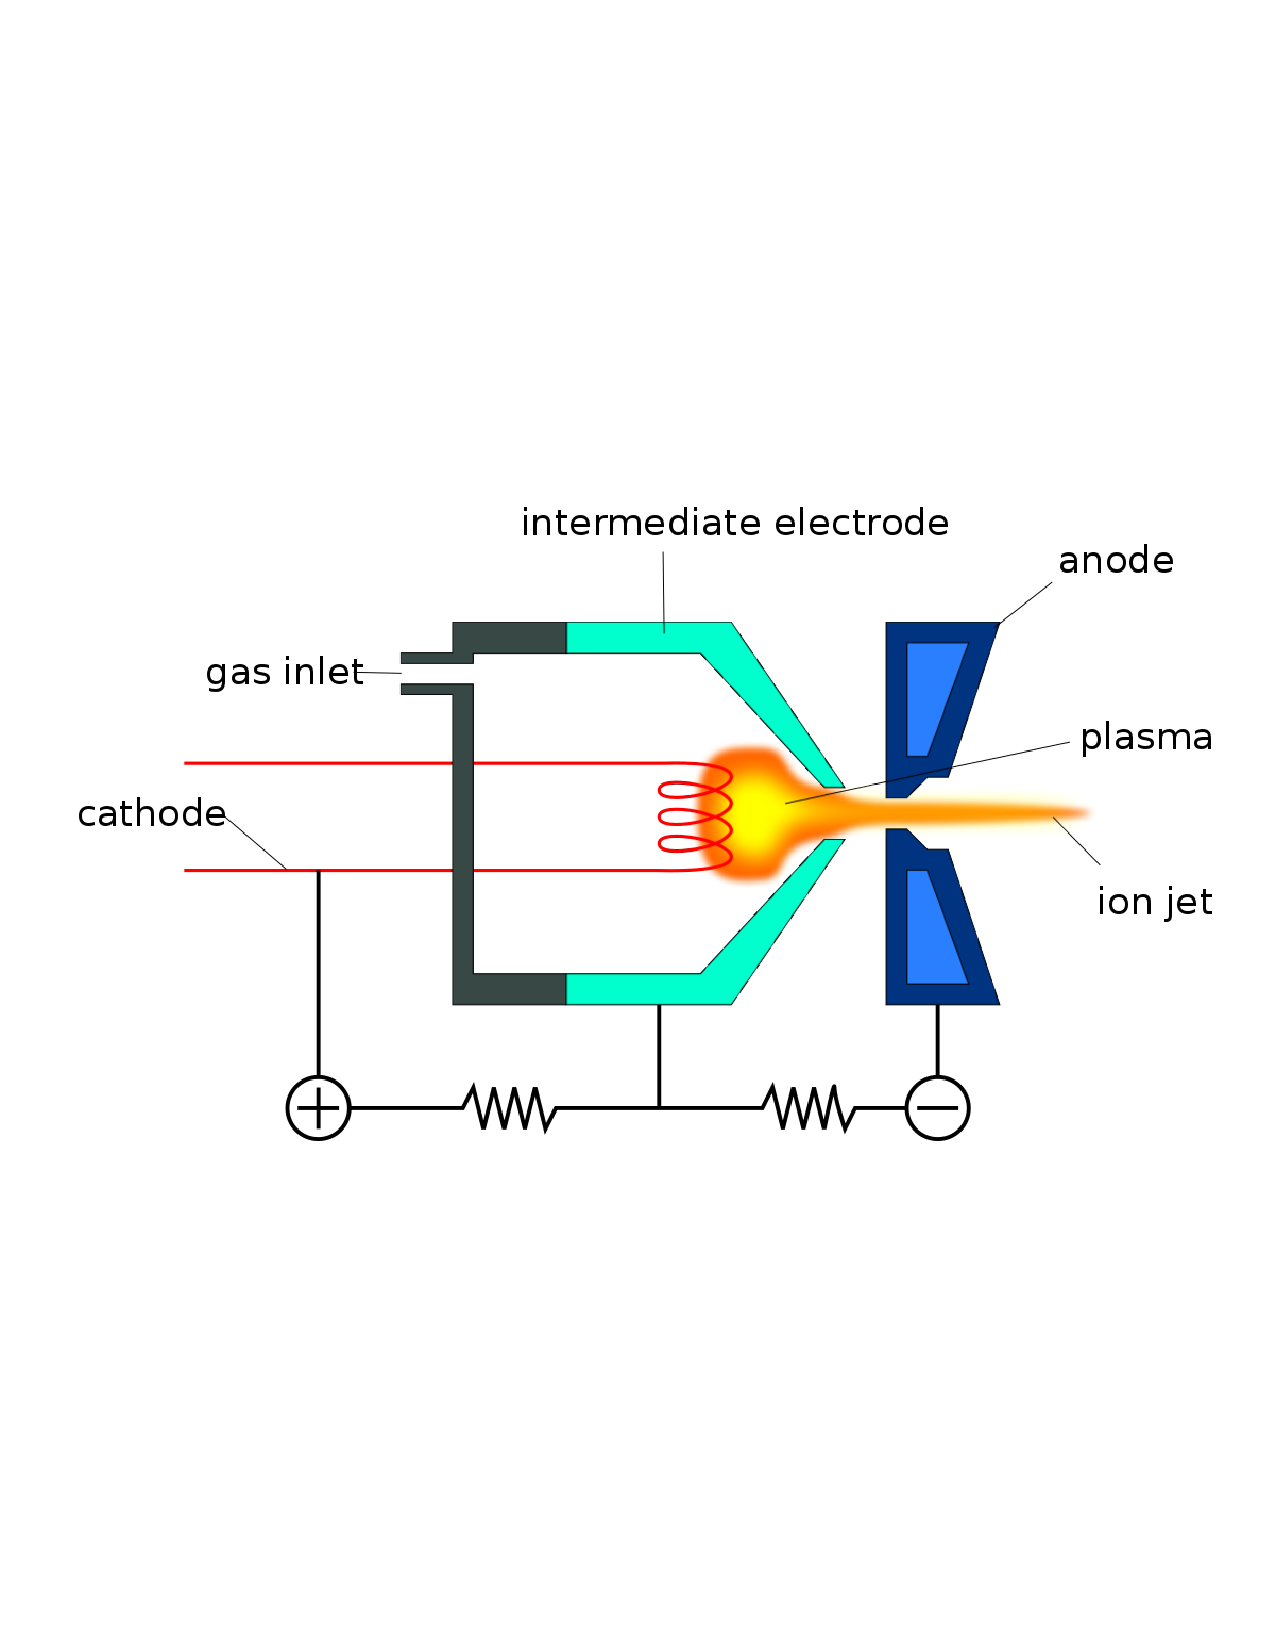
\includegraphics[scale=.3]{duoplasmatron.pdf}
	\caption{Duoplasmatron. Credit: }
\end{figure}

\end{frame}


\begin{frame}
	\frametitle{Path of a Proton at the LHC}
	
\begin{itemize}
	\item protons enter linac2 and are accelerated by RF cavities
	\begin{itemize}
		\item EM waves are generated using an antenna, the cavity is shaped in a way that allows the em 			waves to resonate
		\item the waves oscillate in phase with the protons so that when it enters each cavity, the protons only 		feel a forward acceleration not a backward acceleration
	\end{itemize}
\end{itemize}

\begin{figure}
	\vspace*{-3.3cm}
	 \hspace*{0cm}
	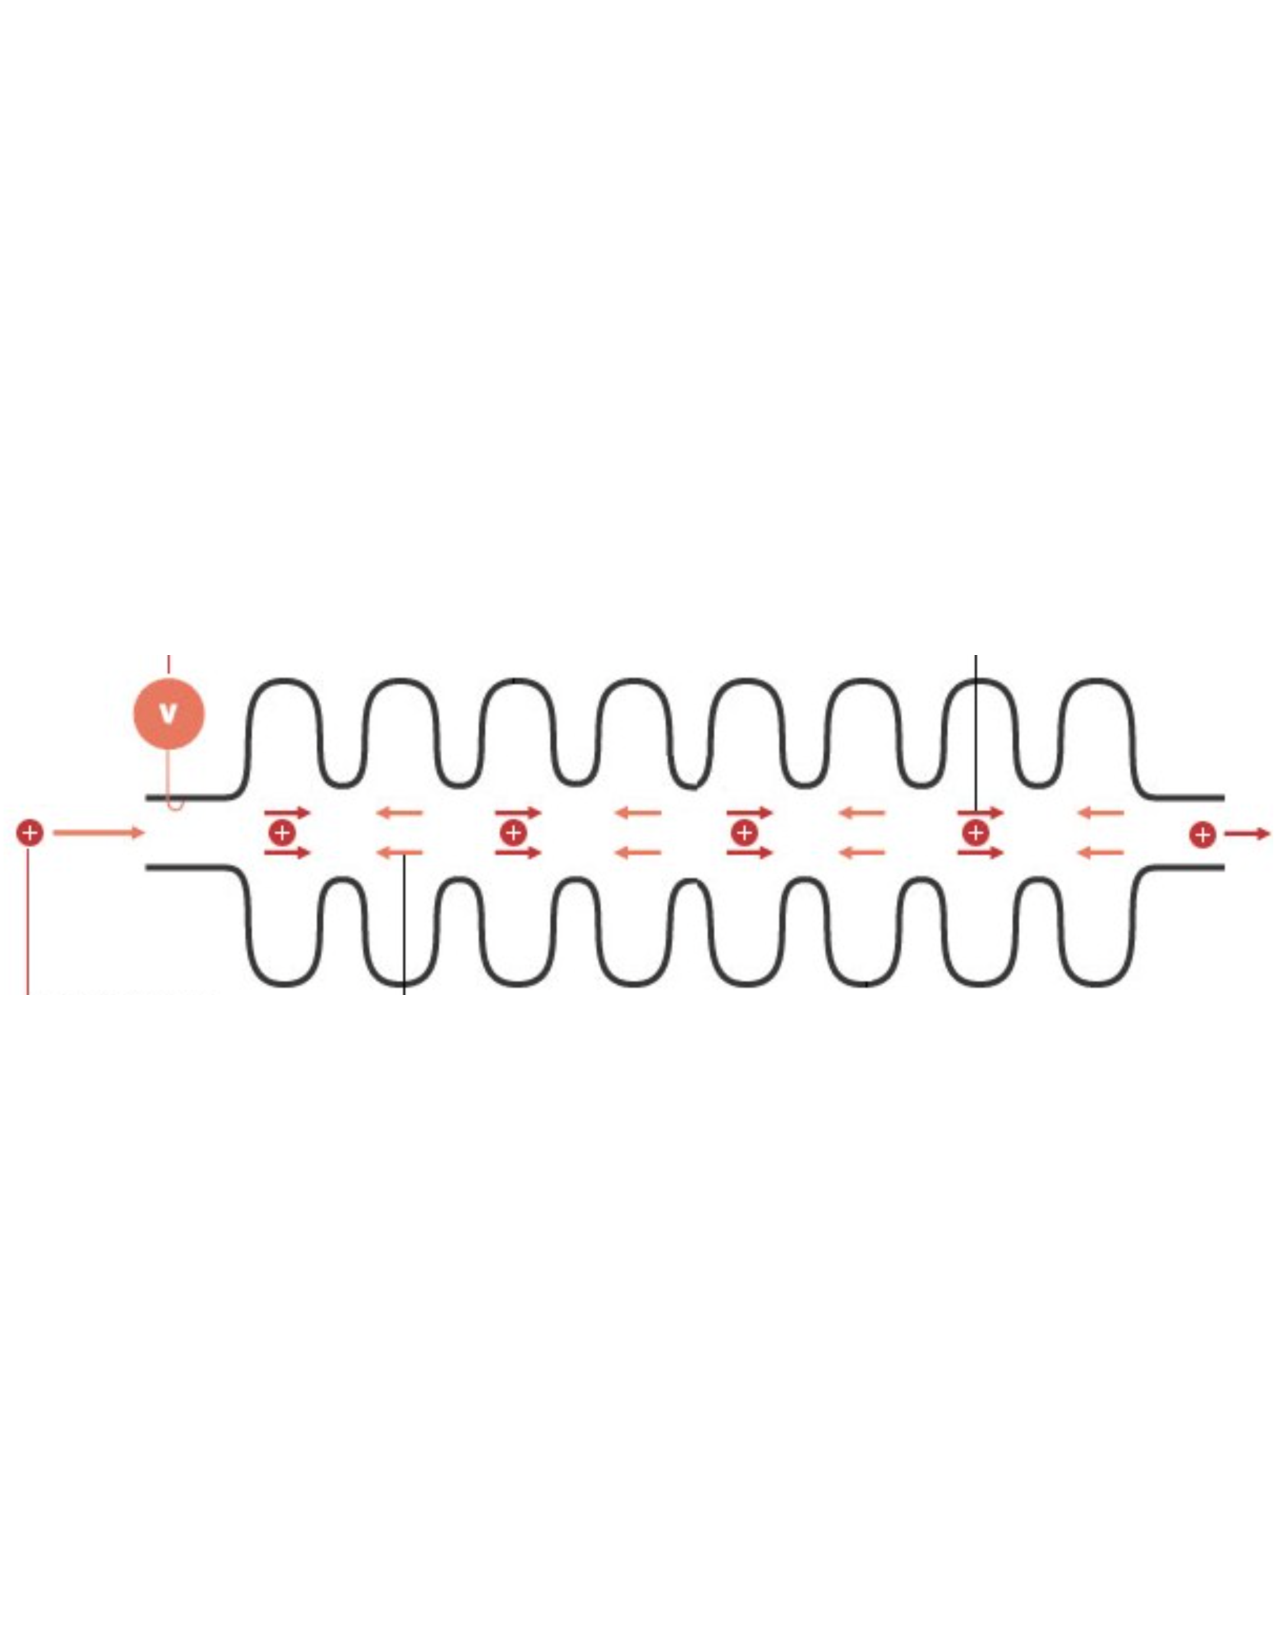
\includegraphics[scale=.3]{rf_cavity.pdf}
\end{figure}

\begin{figure}
	\vspace*{-4.5cm}
	 \hspace*{7cm}
	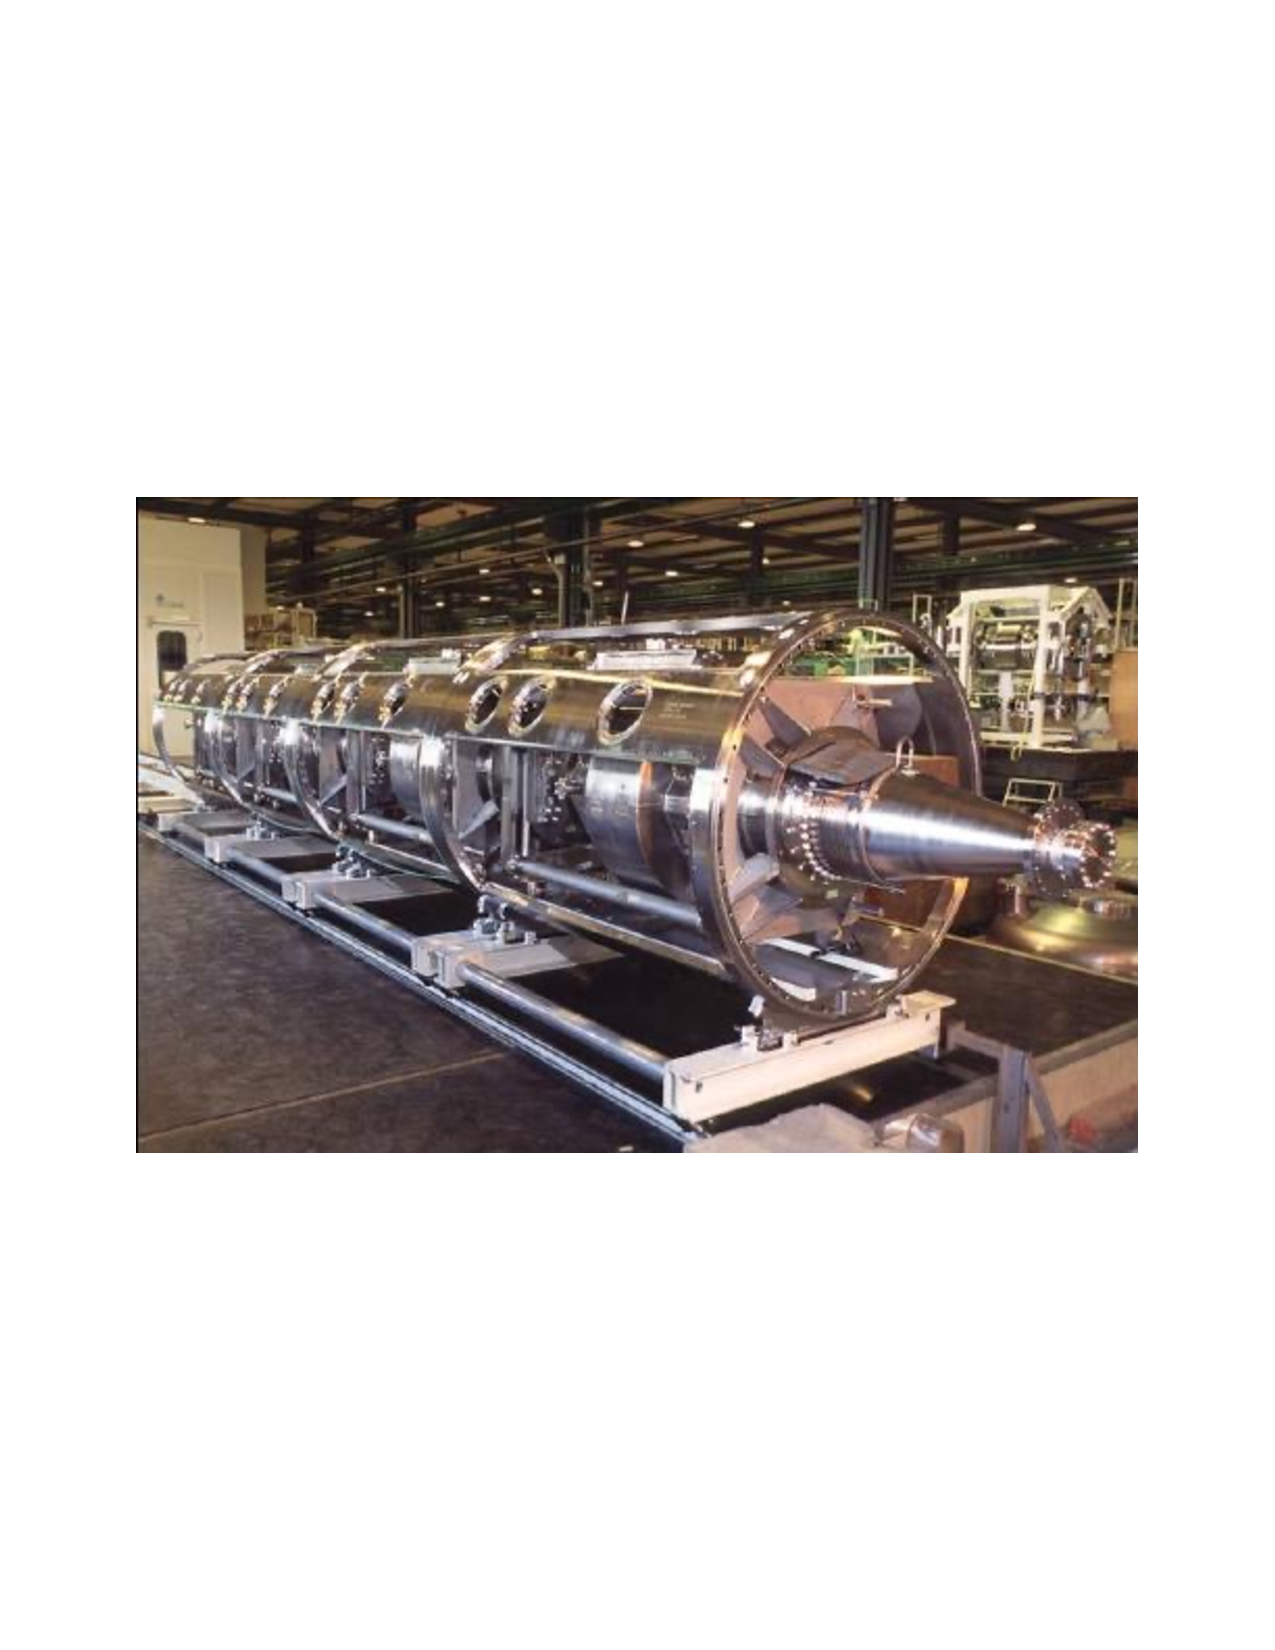
\includegraphics[scale=.2]{rf_cavity_act.pdf}
\end{figure}

\begin{figure}
	\vspace*{-6cm}
	 \hspace*{-7cm}
	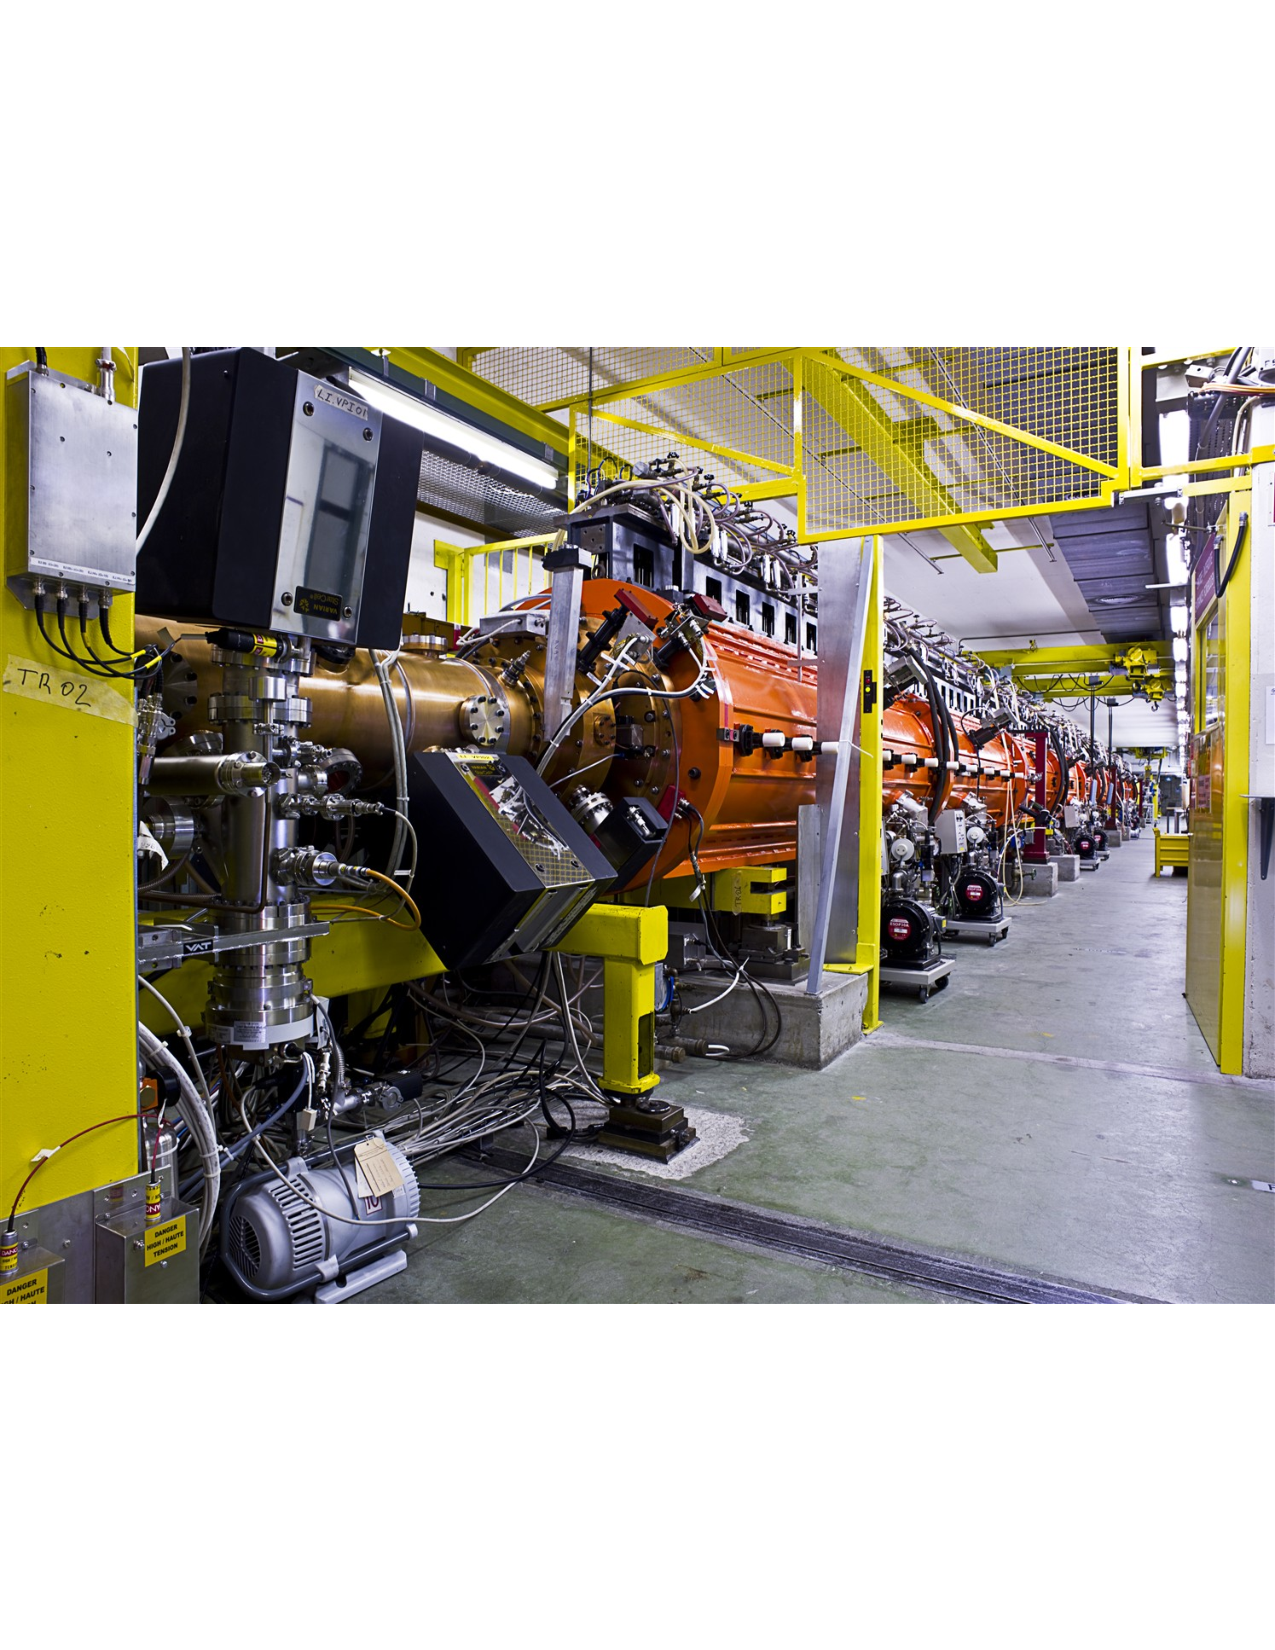
\includegraphics[scale=.2]{linac.pdf}
\end{figure}


\end{frame}


\begin{frame}
\frametitle{Path of a Proton at the LHC}
\begin{itemize}
	\item protons are accelerated into the Proton Synchrotron Booster
	\begin{itemize} 
		\item synchrotrons work very similarly to linear accelerators, they use RF cavities
		\item the major difference is they periodically travel through strong magnetic fields, which keep the 			trajectory in a circle
	\end{itemize}
	\item the protons undergo two more stages of synchrotrons
	\begin{itemize} 
		\item proton synchrotron
		\item super proton synchrotron
	\end{itemize}
\end{itemize}
\begin{figure}
	\vspace*{-2cm}
	 \hspace*{0cm}
	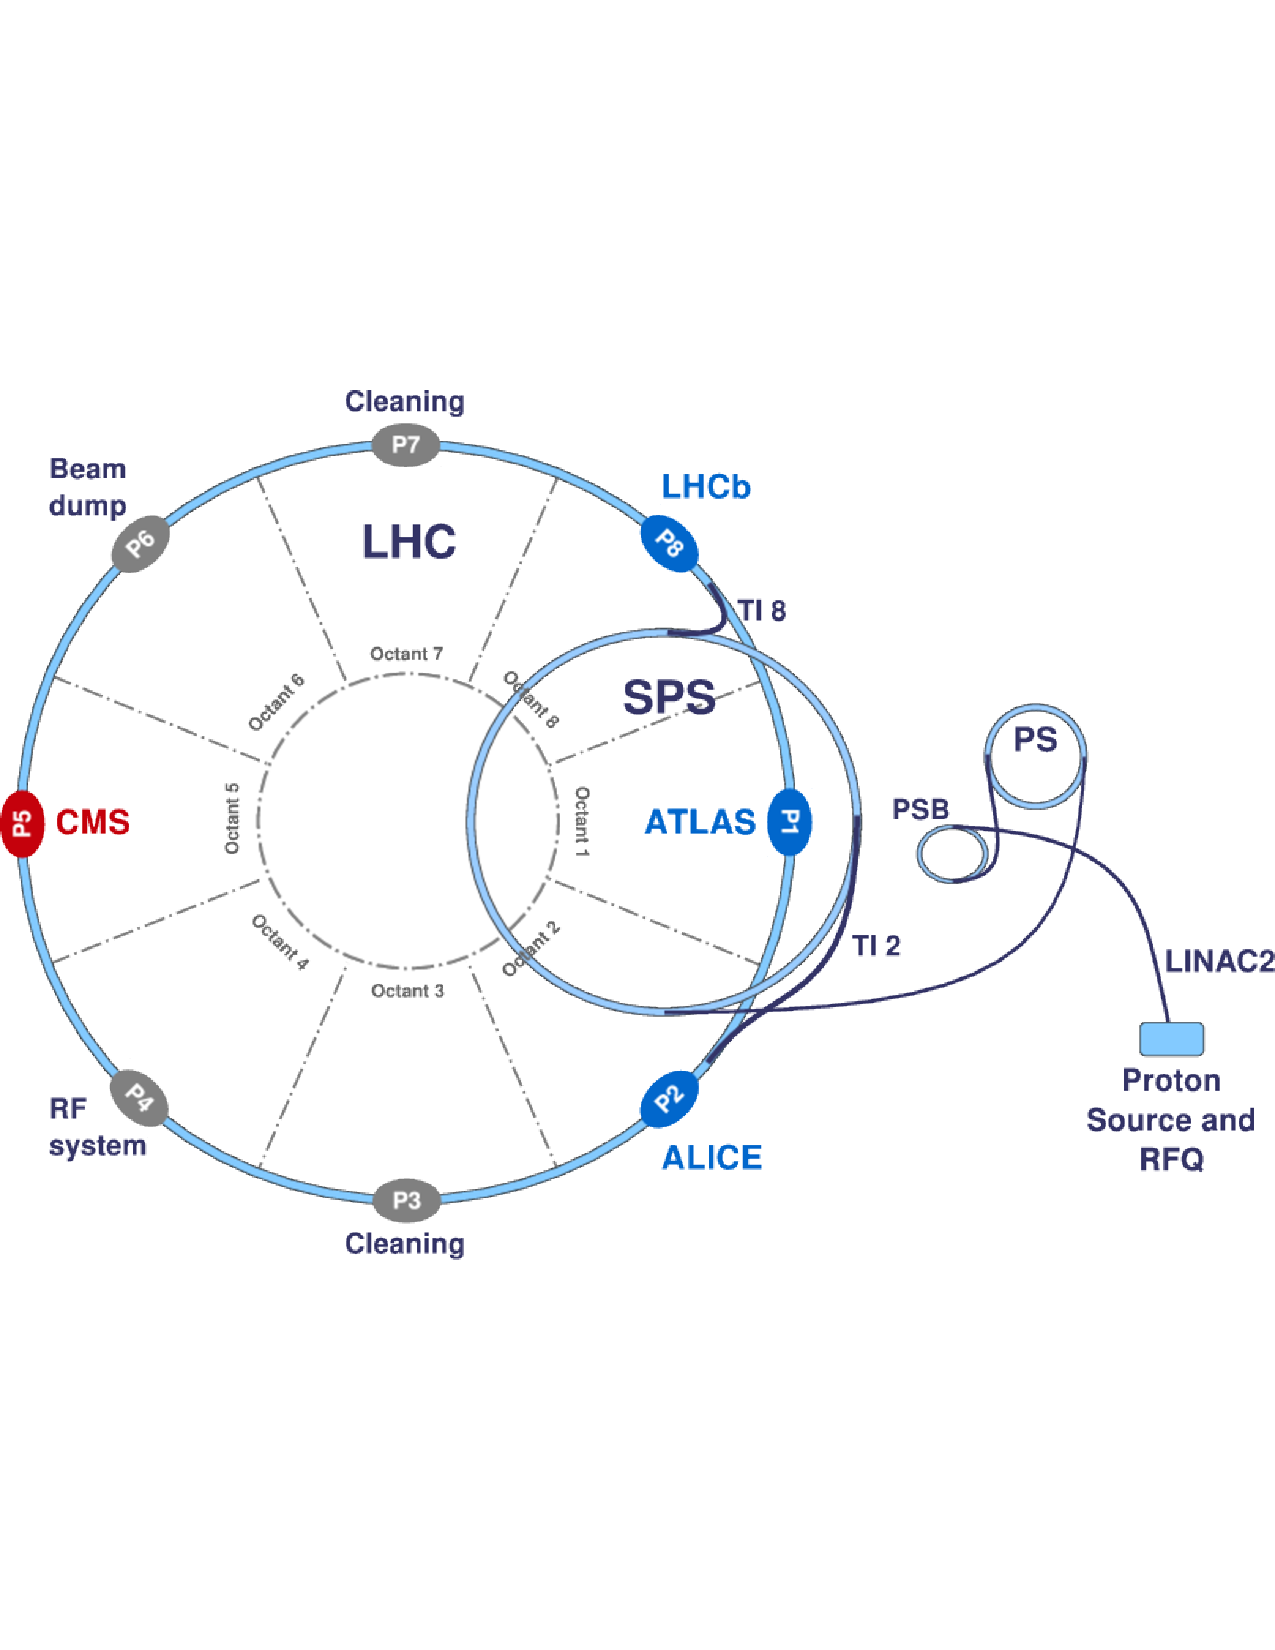
\includegraphics[scale=.3]{cern_map.pdf}
	\caption{Creodocs logo.}
\end{figure}
\end{frame}

\begin{frame}
\frametitle{Last Stage: LHC}
\begin{itemize}
	\item SPS splits the bunches into two beams that are directed into the LHC
	\item Like the synchrotron, LHC uses RF cavities and dipole magnets to accelerate and deflect proton beams

\end{itemize}
\begin{figure}
	\vspace*{-2cm}
	 \hspace*{0cm}
	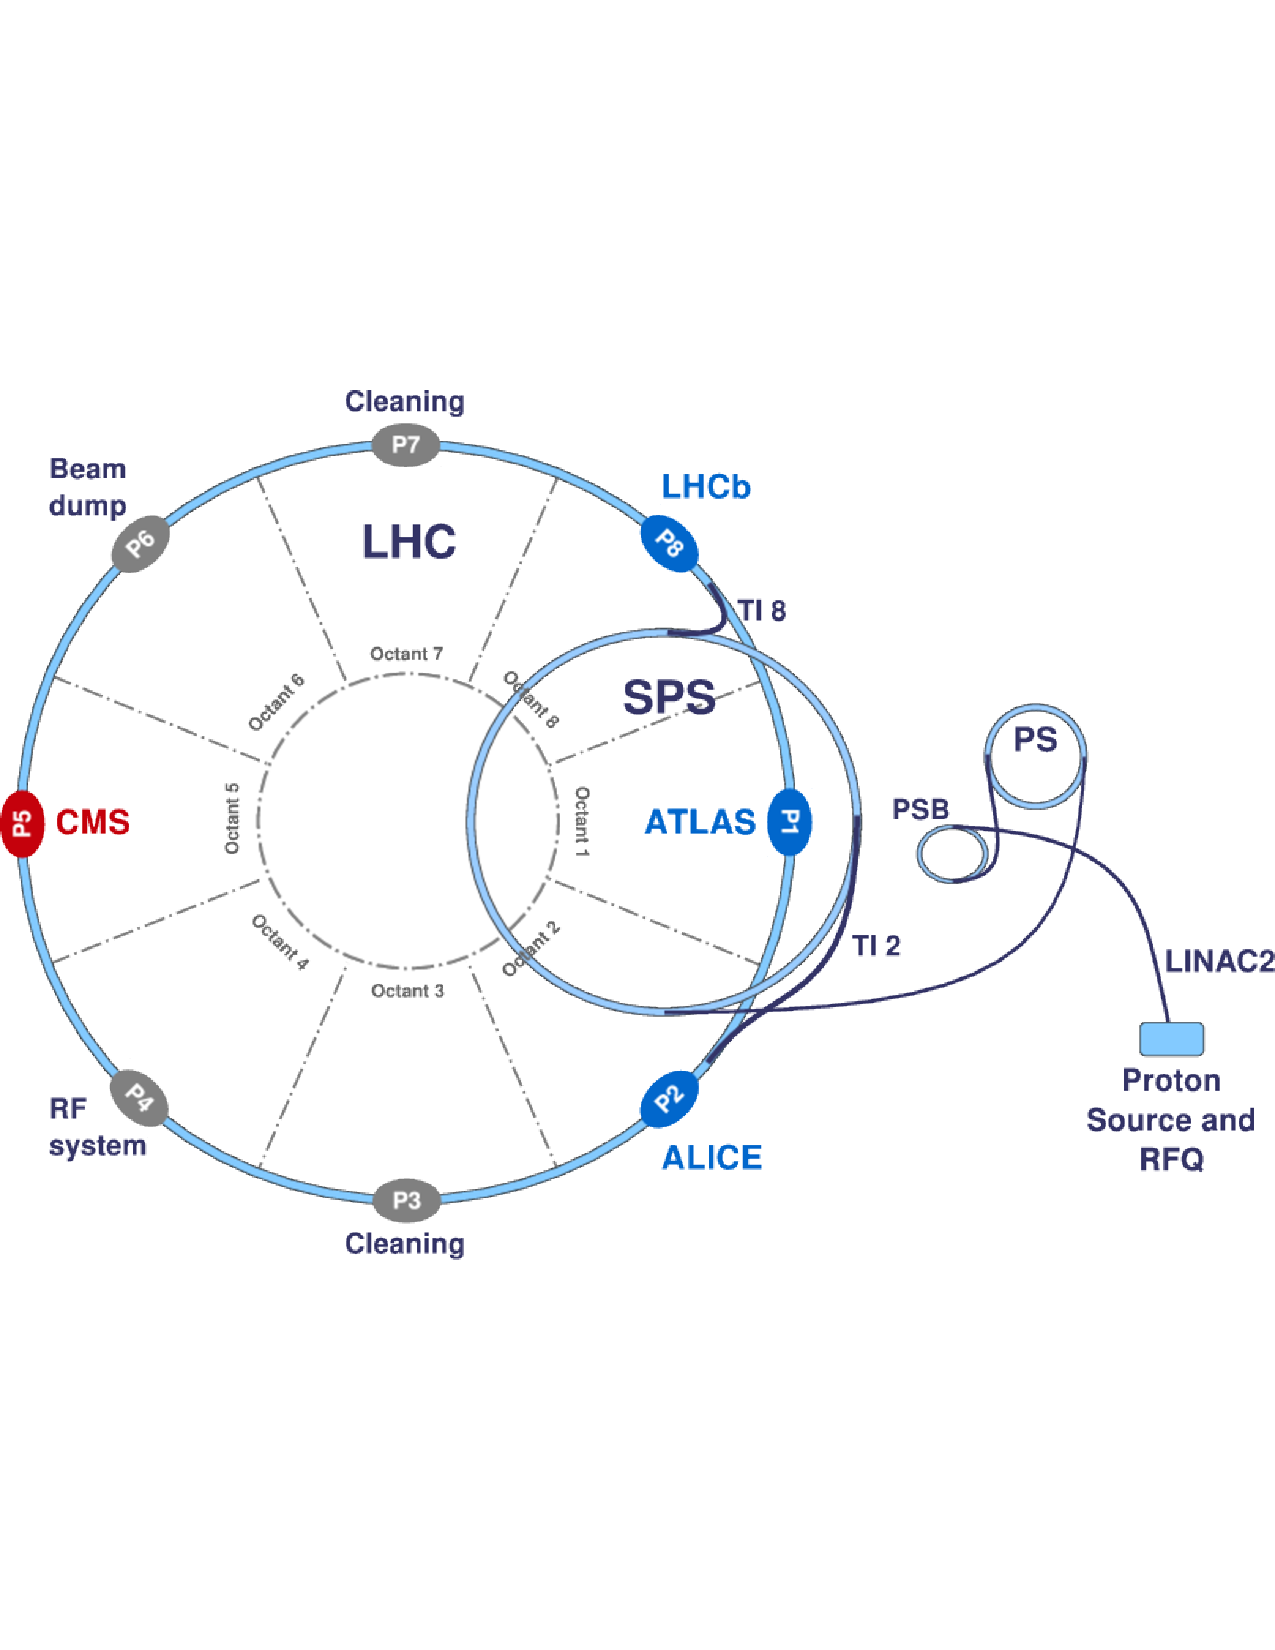
\includegraphics[scale=.3]{cern_map.pdf}
	\caption{Creodocs logo.}
\end{figure}
\end{frame}

\begin{frame}
\frametitle{Interesting Facts}
\begin{itemize}
	\item full capacity is ~2800 bunches, spaced roughly 7 m apart
	\item each bunch is about 30 cm in length
	\item initially the beam diameter is about a milimeter
	\item each proton is accelerated to an energy of 7 TeV
		\begin{itemize}
			\item at this energy, the observed mass fo the proton is 7000 times heavier than it is at rest
		\end{itemize}
	\item this is roughly the same as the kinetic energy of a flying mosquito
	\item if the mosquito had the same energy density of the proton...
	\begin{itemize}
%Energy density of that proton 2.677*10^(38) j/m^3
%Energy released by nuclear bomb 1.5*10^13 joules
%Volume of 1 cm mosquito 10**-6
%If the mosquito had the same energy density of the proton, it would have the same amount of energy at %1.7*10^19 Hiroshima nuclear bombs.
%Assuming a radius of 2 meters for the nuke roughly 12 m^2 area
%The mosquito would have the same amount of energy as a lot of nukes, enough to cover the entire earth… 408,000 times! This would reach a height of a low orbit satellite!
		\item the mosquito would contain the same amount of energy released in $1.7 \times 10^{19}$ nuclear bombs
		\item assuming a diameter and height of 2 m for each nuke, this is enough nukes to cover the entire earth... 400,000 times
		\item this would reach a height of a low orbit satellite!
		\end{itemize}

\end{itemize}

\end{frame}

\begin{frame}
\frametitle{Intersecting the Beams}
	\begin{itemize}
		\item beams are focused at one of the detectors and deflected so they intersect
			\begin{itemize}
				\item beams are focused to 60 microns, or roughly the width of a human hair
				\item even with ~2800 bunches there are only ~20 proton collisions per passing
			\end{itemize}
	\end{itemize}

\begin{figure}
	\vspace*{-2cm}
	 \hspace*{0cm}
	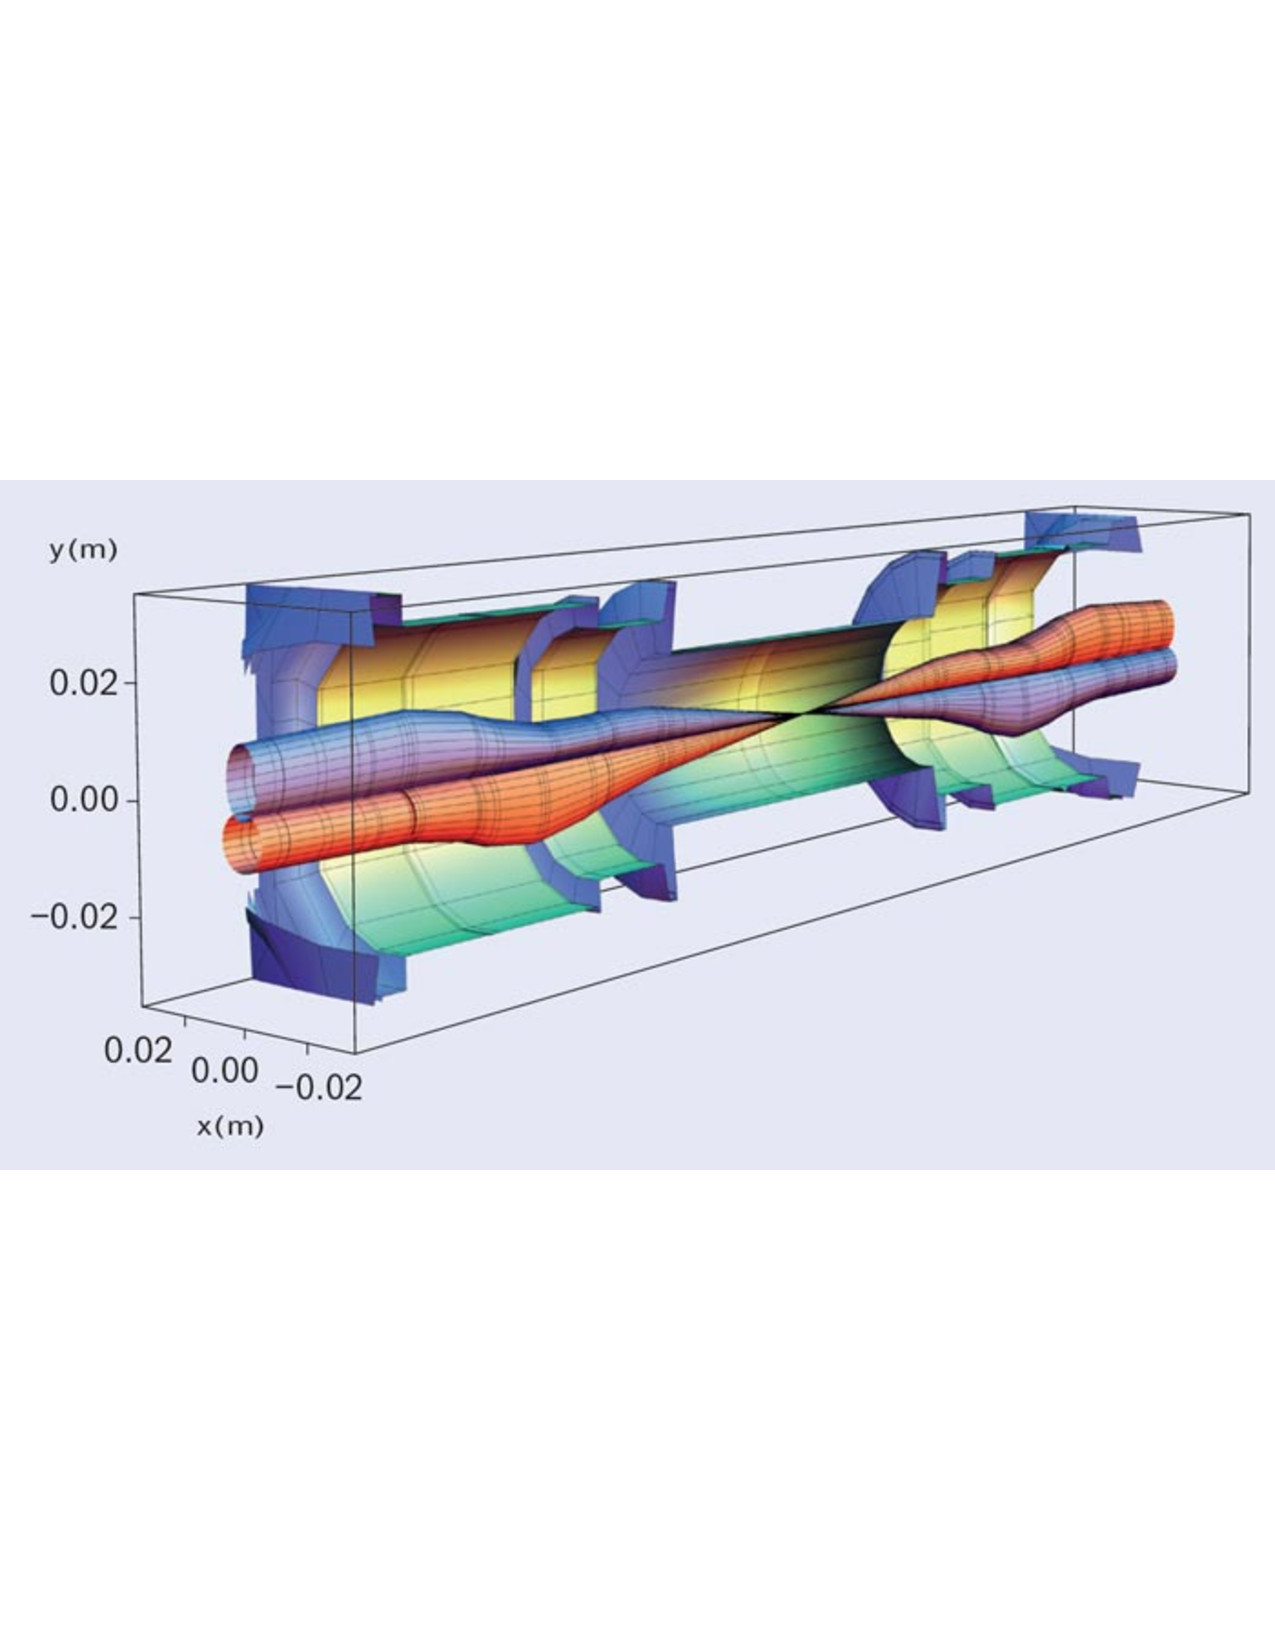
\includegraphics[scale=.3]{beams.pdf}
	\caption{Creodocs logo.}
\end{figure}
\end{frame}

\begin{frame}
\frametitle{Example of Colliding Protons}
	\begin{itemize}
		\item an extremely simple example of how protons may collide inelastically
		\item examples are generally much more complicated and can produce hundreds of outgoing particles
	\end{itemize}
	
\begin{figure}
	\vspace*{-2cm}
	 \hspace*{-5cm}
	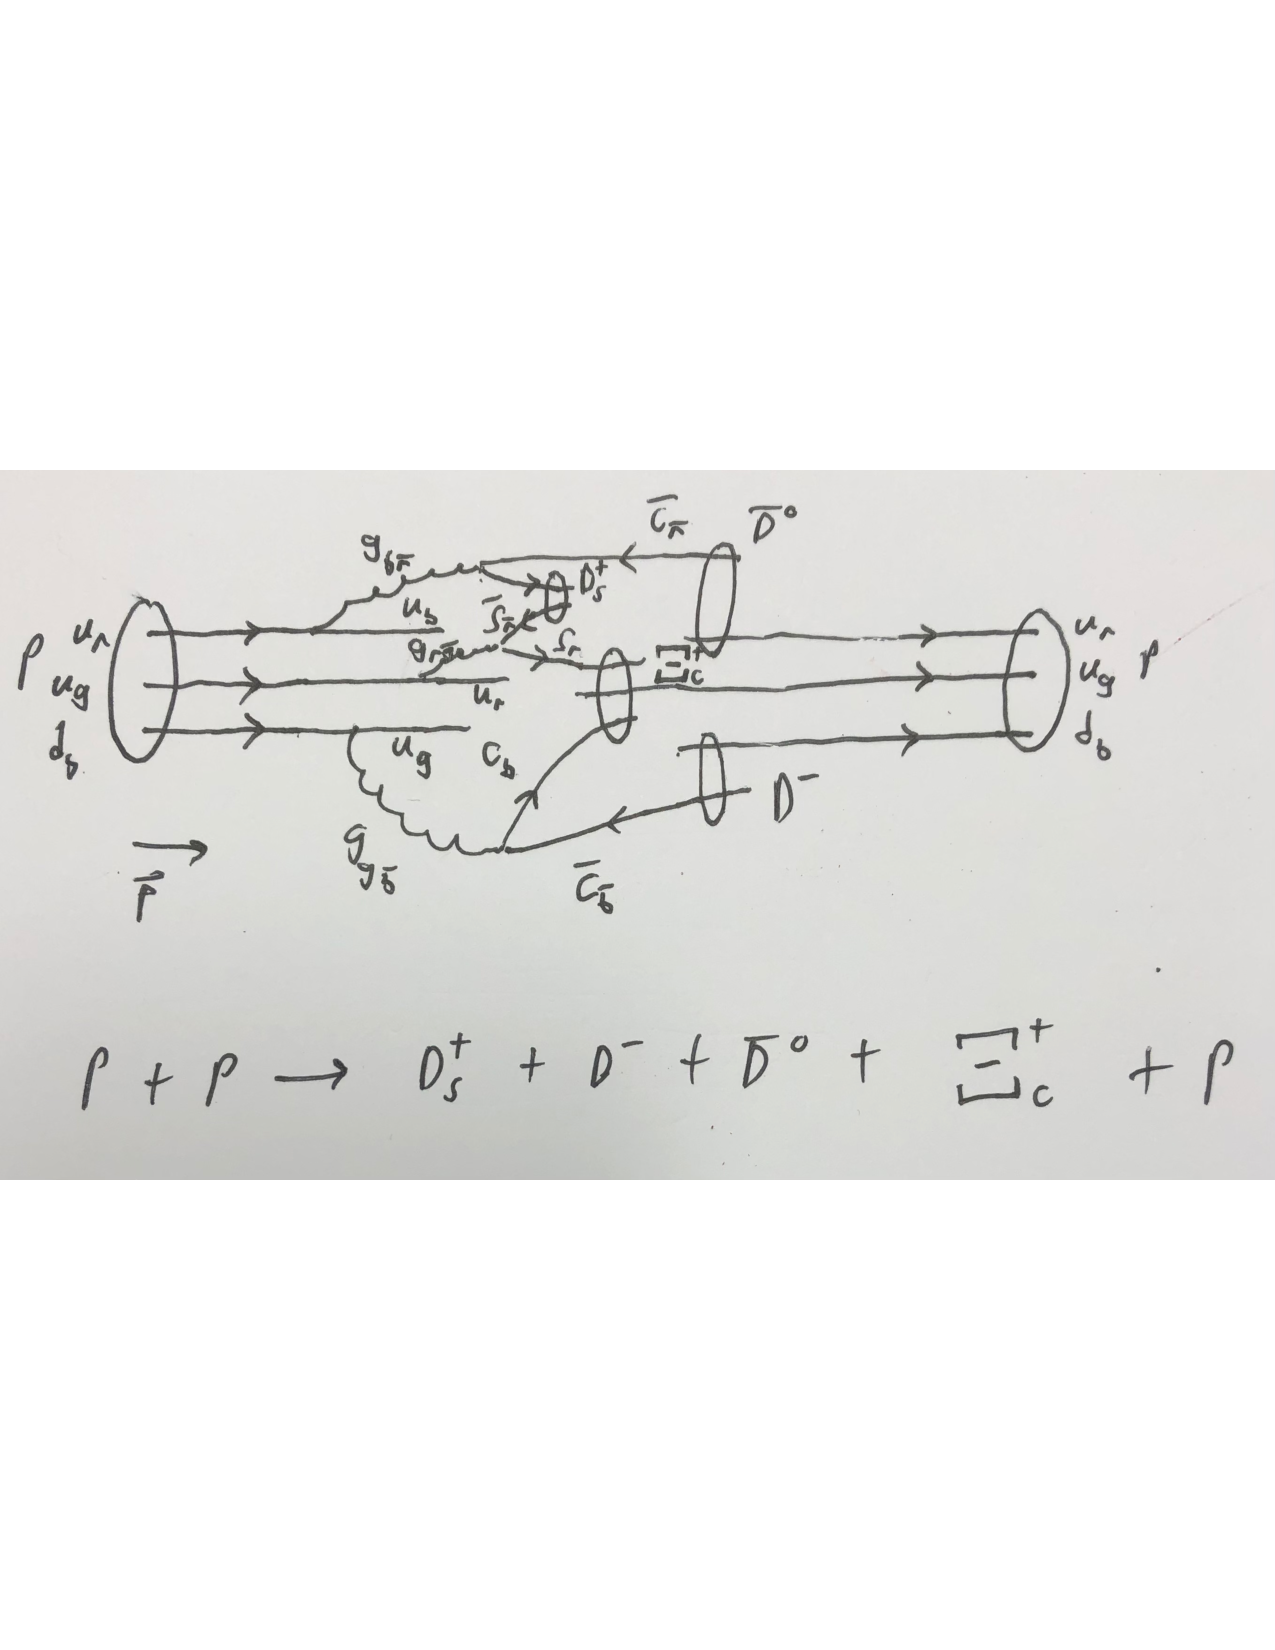
\includegraphics[scale=.3]{proton_collision.pdf}
\end{figure}
%I believe this is a hard scattering process, we need to include the strange ways that they can collide, like soft processes and quark gluon plasma.
\begin{figure}
	\vspace*{-8cm}
	 \hspace*{6cm}
	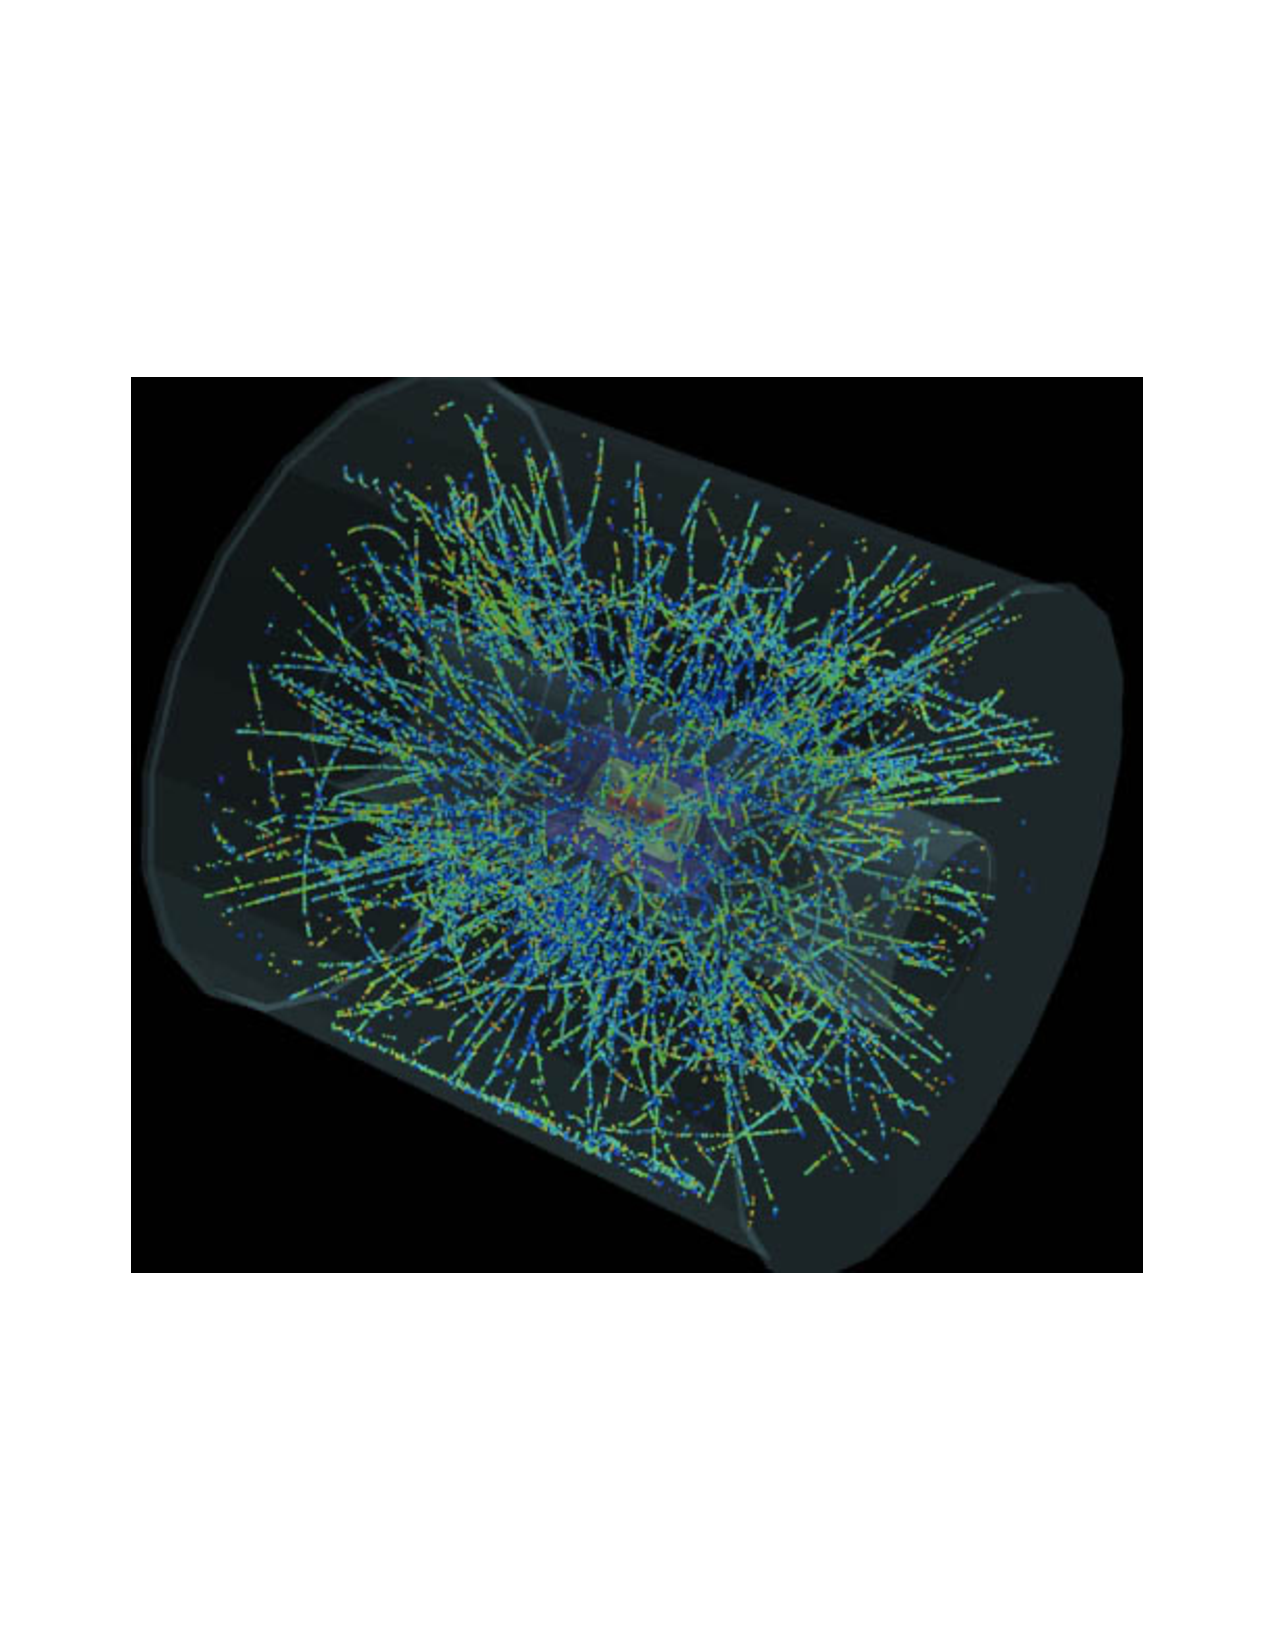
\includegraphics[scale=.2]{cern_collision.pdf}
\end{figure}
\end{frame}


\begin{frame}
\frametitle{Motivation for FASER}
	\begin{itemize}
		\item as can be seen from the atlas detector a lot of effort is put into detecting particles in the transverse direction
		\item not a lot of effort is put into searching for particles in the tangential (forward) direction
		\item enter ForwArd Search ExpeRiment (FASER)
	\end{itemize}
\begin{figure}
	\vspace*{-2cm}
	 \hspace*{0cm}
	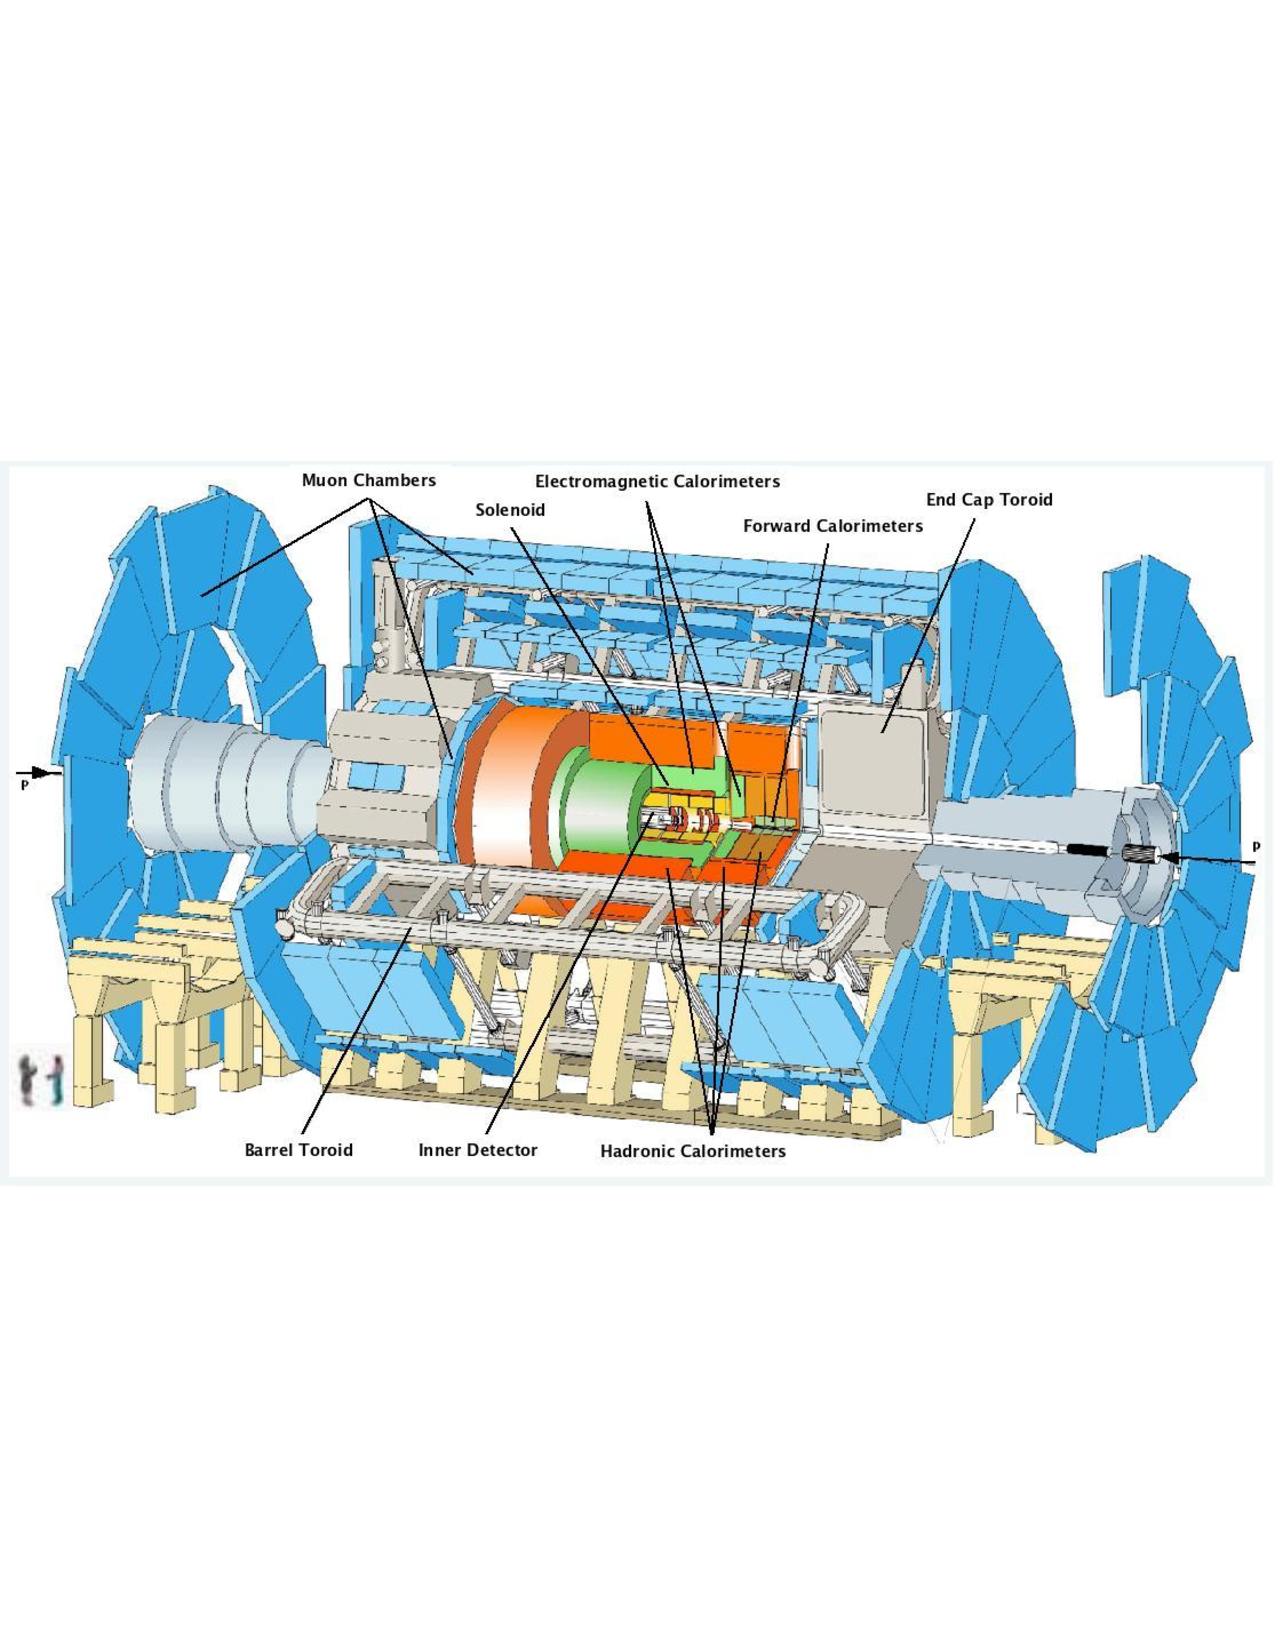
\includegraphics[scale=.3]{atlas.pdf}
\end{figure}
\end{frame}


\begin{frame}
\frametitle{FASER}
	\begin{itemize}
		\item FASER is located 480 m from the ATLAS detector in the forward direction
		\item it is designed to search for particles that are barely deflected after collisions
		\begin{itemize}
			\item searches for particles such as dark photons, axion-like particles, sterile neutrinos, etc.
		\end{itemize}
		\item it is an emulsion detector and measures energy of the particle
		\item we will focus on my research which involves a special type of sterile neutrino called heavy neutral leptons (HNL)
		\item to figure out if we have discovered a new particle we must compare with theory
		\item we must simulate this experiment... Enter FORward Experiment SEnsitivity Estimator (FORESEE)

		%but the mesons that produce the weak particles can be deflected strongly, so why is this useful?
	\end{itemize}
\end{frame}





\begin{frame}
\frametitle{FORESEE Motivation}
	\begin{itemize}
		\item FASER uses an emulsion detector, which detects the tracks of charged particles
			\begin{itemize}
				\item this means HNL cannot be detected with these detectors
				\item HNL's have a lifetime and can decay into standard model particles, and these can interact with the detector
			\end{itemize}
		\item these detectors measure energy 
		\item we can extract N(E) from experiment, the number of particles as a function of energy
			\begin{itemize}
				\item this will give us the total number of particles as a function of energy, so to get the signal we are interested in we must subtract all known interactions to obtain the interesting portion
%need to understand how we can find N(E) for all particles that HNLs decay into 
				\item it is this distribution that we can compare with theory
			\end{itemize}
		\item this analysis tells us we need FORESEE to produce $N_{HNL}(E)$ for HNL's
			\begin{itemize}
				\item but first lets understand HNL's
			\end{itemize}
	\end{itemize}
\end{frame}


\begin{frame}
\frametitle{Heavy Neutral Leptons (HNLS)}
	\begin{itemize}
		\item the theory of HNL's is given by
		\begin{itemize}
			\item $\mathcal{L}_{HNL} = \frac{1}{2} \bar{N}_m \slashed{\partial}N_m - \frac{1}{2} M_m \bar{N}_m N_m - \frac{1}{2} m_{ab} \bar{\nu}_a \nu_b - F_{am} \bar{L}_a N_m \tilde{\phi}$
		\end{itemize}
			\begin{itemize}
				\item where $N$ is a $SU(3) \times SU(2) \times U(1)$ singlet 
				\item $\nu \sim$ standard model (SM) neutrinos
				$L = \begin{pmatrix} \nu \\ \ell \end{pmatrix},\,\,$ SM SU(2) doublet
					\begin{itemize}
					\item  $\ell ~ $SM lepton
					\end{itemize}
				\item $\phi$ Higgs SU(2) doublet
			\end{itemize}
		\item can be rewritten as $\mathcal{L}_{HNL}= \frac{1}{2} \bar{N}_m \slashed{\partial} N_m - \frac{1}{2} \begin{pmatrix} \bar{\nu} & \bar{N} \end{pmatrix} \begin{pmatrix} m & \mu \\ \mu^T & M \end{pmatrix} \begin{pmatrix} \nu \\ N \end{pmatrix}$
			\begin{itemize}
				\item we assume $M>>\mu>>m \approx 0$
			\end{itemize}
		\item can be diagonalized (to get rid of cross terms)
		\begin{itemize}
			\item $\mathcal{L}_{HNL} \supset - \frac{1}{2} \begin{pmatrix} \bar{\nu}' & \bar{N}' \end{pmatrix} \begin{pmatrix} -\mu^T M^{-1} \mu & 0 \\ 0 & M \end{pmatrix} \begin{pmatrix} \nu' \\ N' \end{pmatrix}$
			\item this is the seesaw mechanism
			\item $\nu' = \nu - U N$
		\end{itemize}
	\end{itemize}
\end{frame}


\begin{frame}
\frametitle{Heavy Neutral Leptons (HNLS)}
	\begin{itemize}
		\item $- \frac{1}{2} \bar{L}_m \slashed{D} L_m$ leads to terms like 
		\begin{itemize}
			\item $\frac{i g_2}{\sqrt{2}} W_{\mu}^+ ( \bar{\nu}_m \gamma^{\mu} e_m)=\frac{i g_2}{\sqrt{2}} W_{\mu}^+ ( \bar{\nu}'_m \gamma^{\mu} e_m) + \frac{i g_2}{\sqrt{2}} W_{\mu}^+ U_{mn} ( \bar{N}_n \gamma^{\mu} e_m)$
		\end{itemize}
		\begin{itemize}
			\item these are Feynman diagram vertices, this allows N to interact with standard model particles
			\item the reason for this amazing effect can be attributed to the Higgs term in the Lagrangian and this is what allows these particles to be detectable 
		\end{itemize}
\begin{figure}[h!]
	\vspace*{0cm}
	 \hspace*{7cm}
	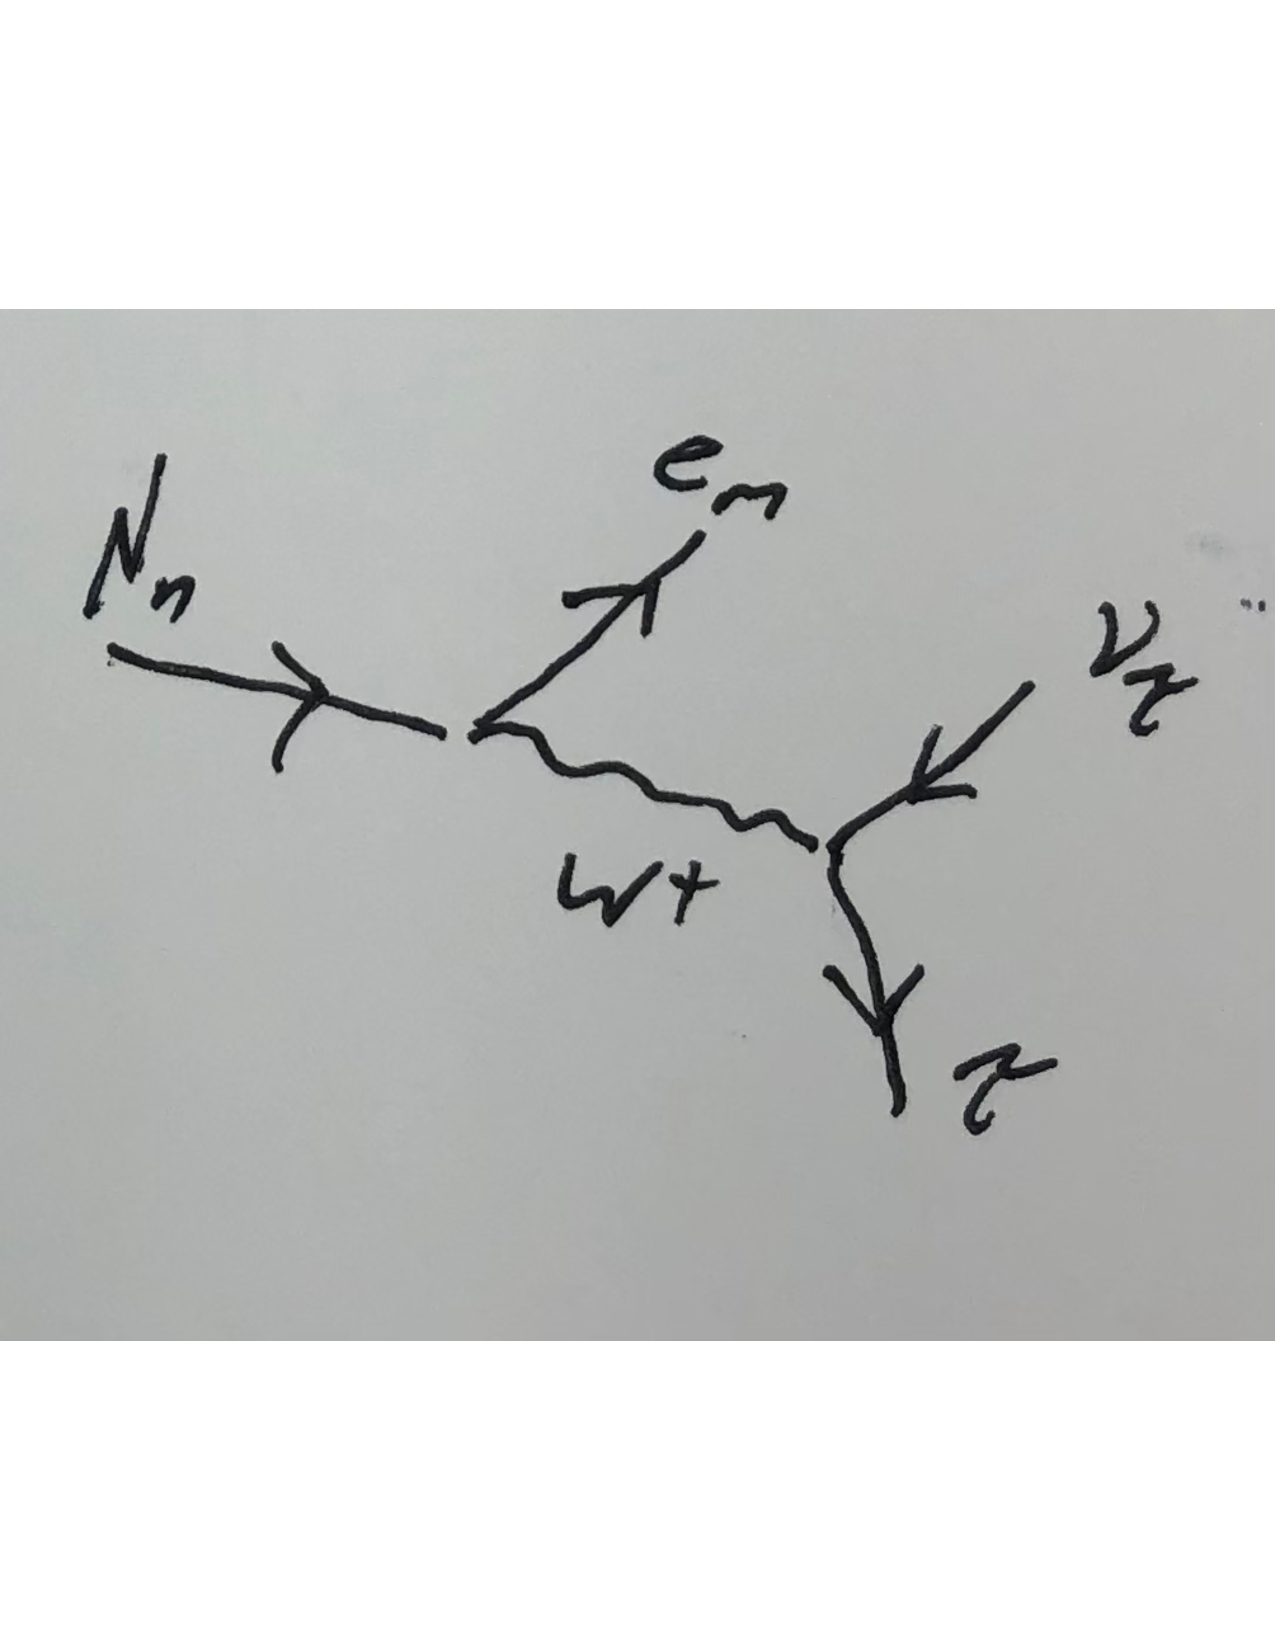
\includegraphics[scale=.1]{Ndecay.pdf}
\end{figure}
\begin{figure}[h!]
	\vspace*{-3cm}
	 \hspace*{-7cm}
	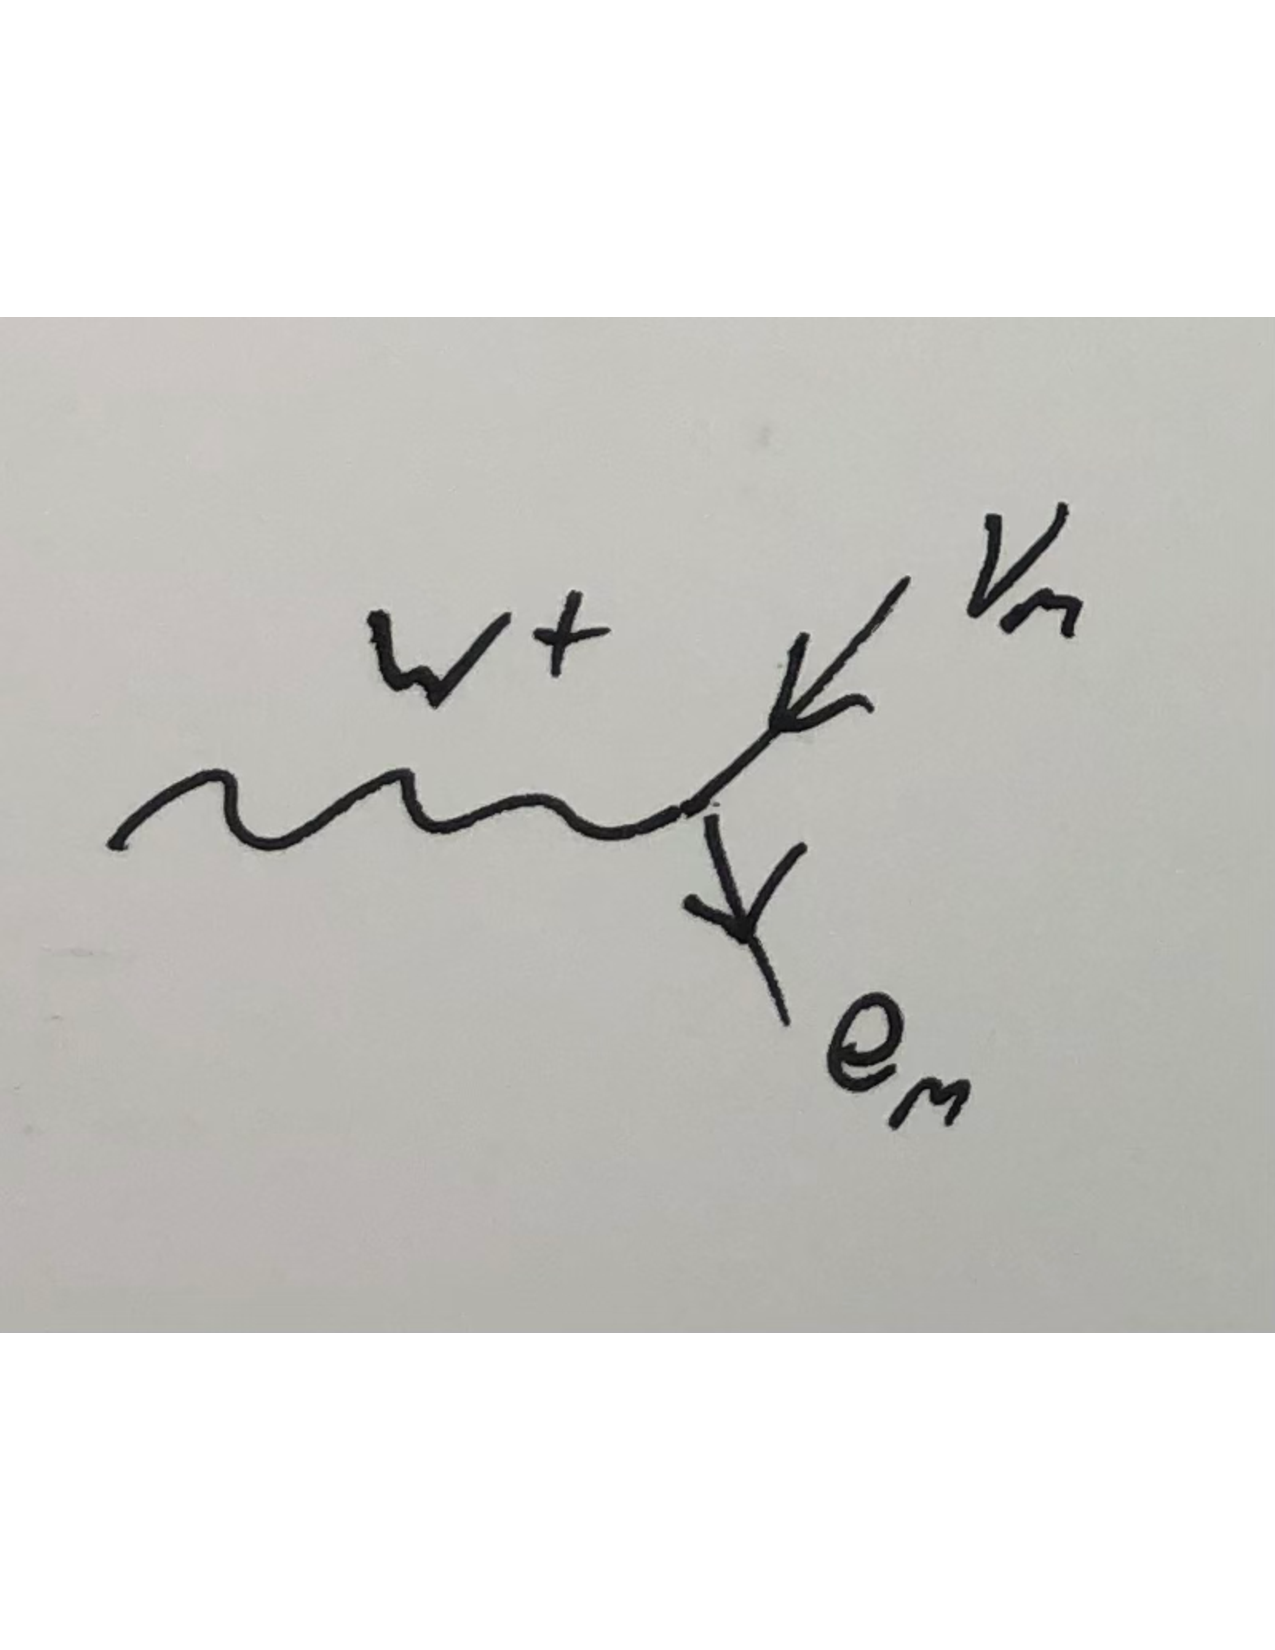
\includegraphics[scale=.1]{nu_e.pdf}
\end{figure}
\begin{figure}
	\vspace*{-3cm}
	 \hspace*{0cm}
	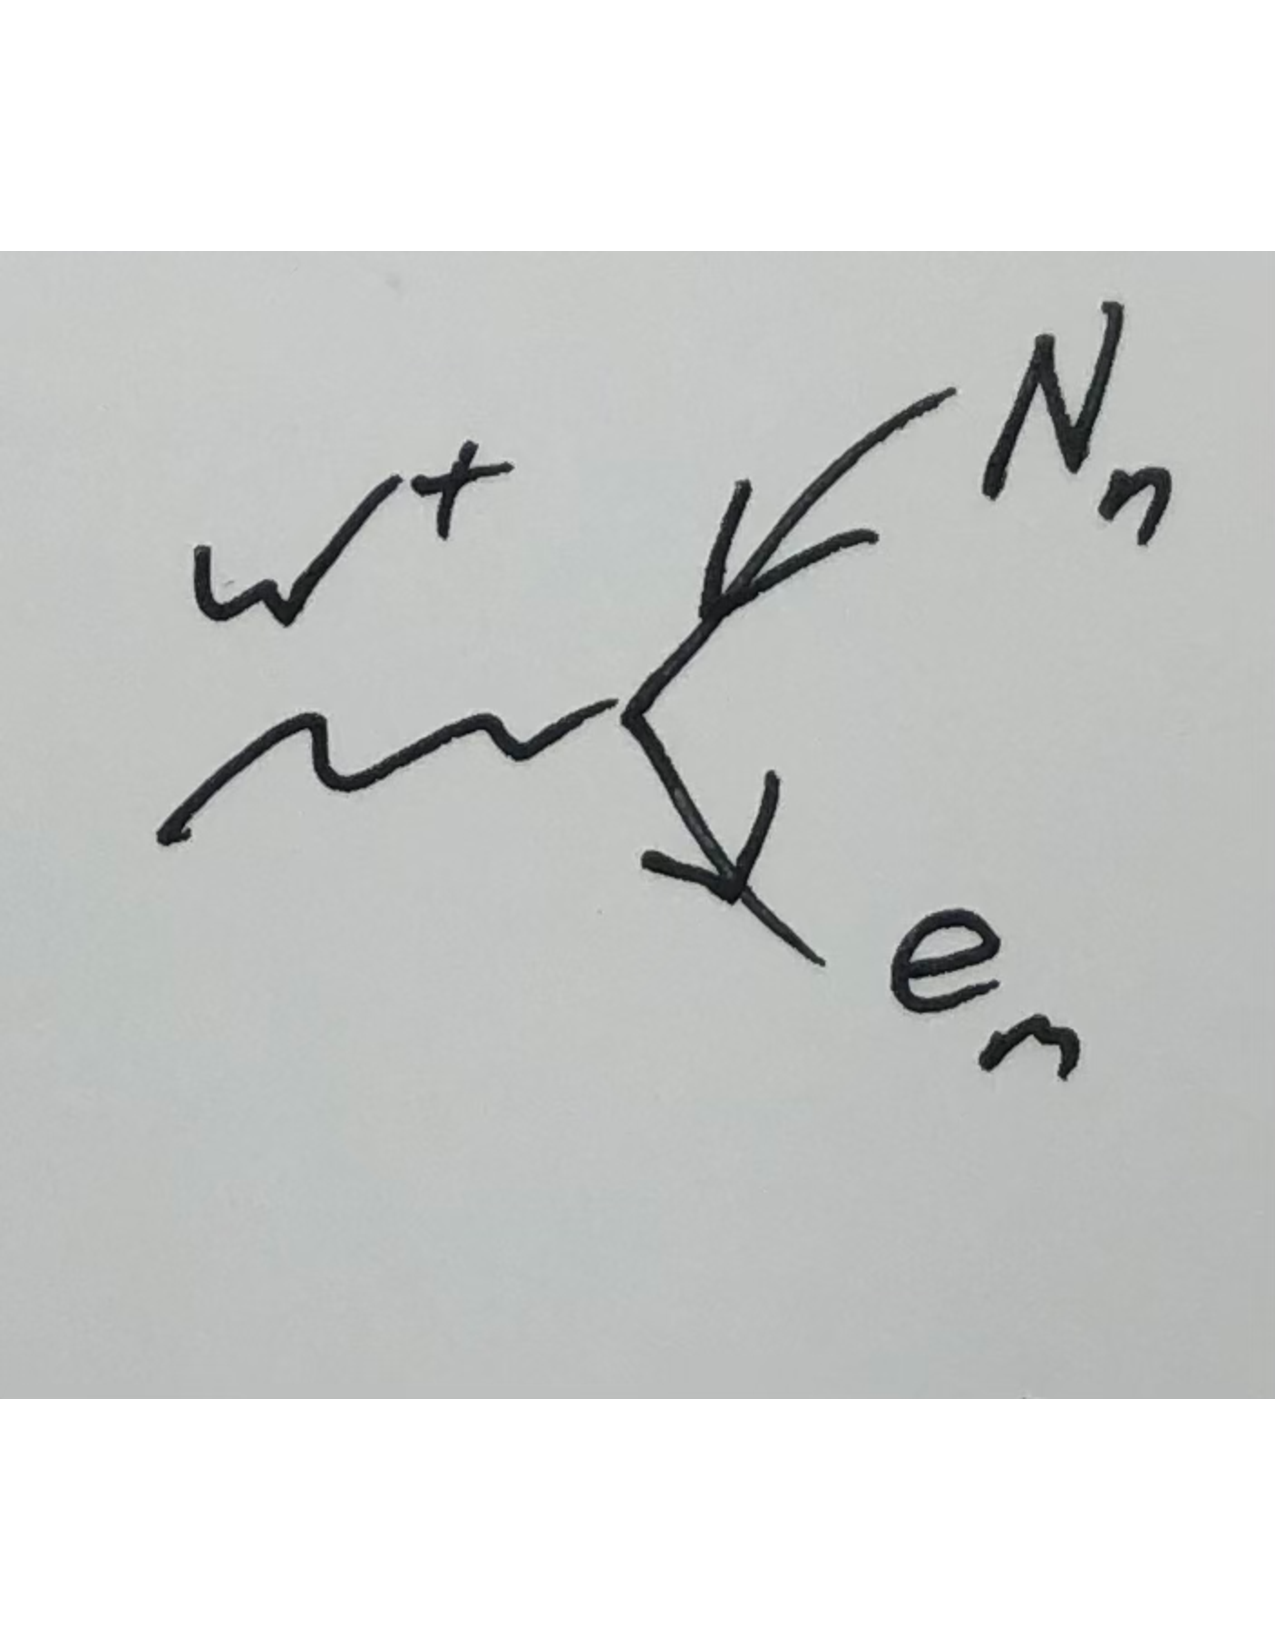
\includegraphics[scale=.1]{N_e.pdf}
\end{figure}
	\end{itemize}
\end{frame}


\begin{frame}
\frametitle{All Together Now}
\begin{figure}
	\vspace*{-1cm}
	 \hspace*{-0cm}
	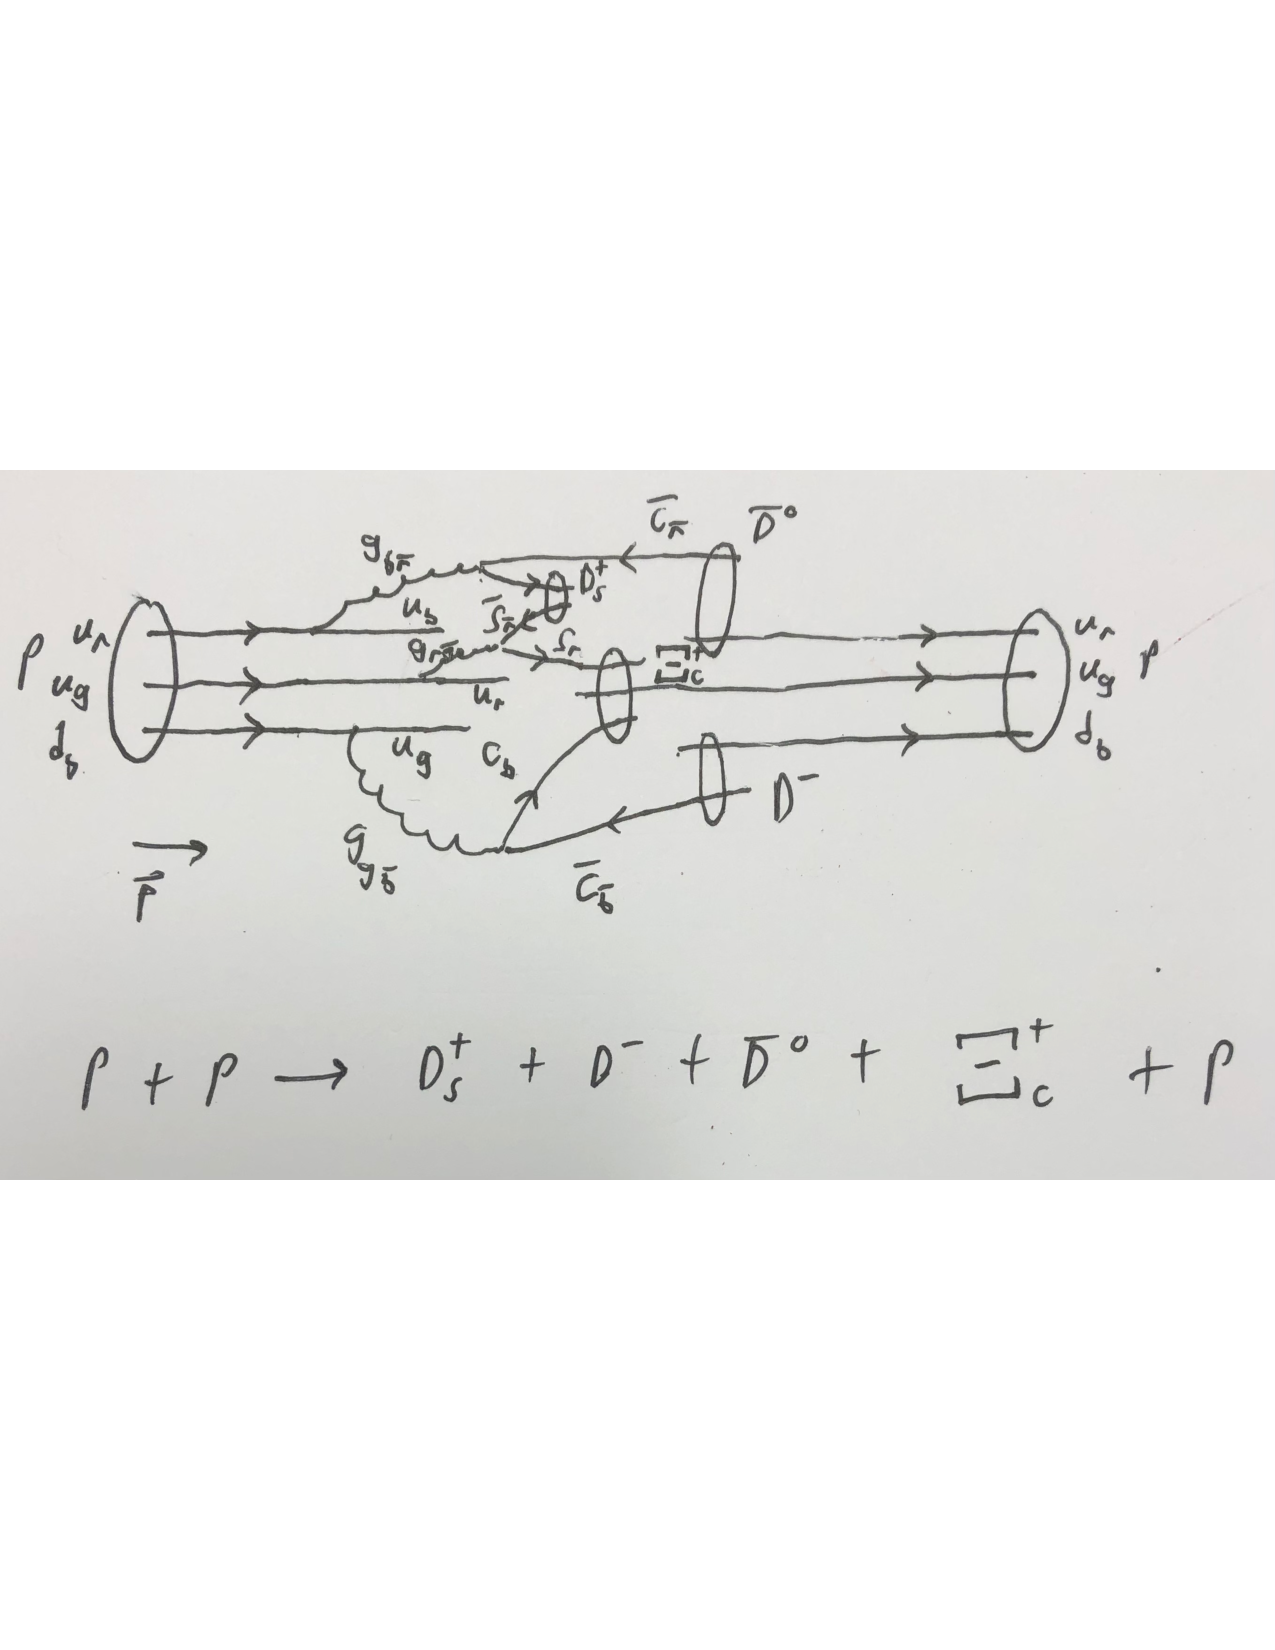
\includegraphics[scale=.18]{proton_collision.pdf}
	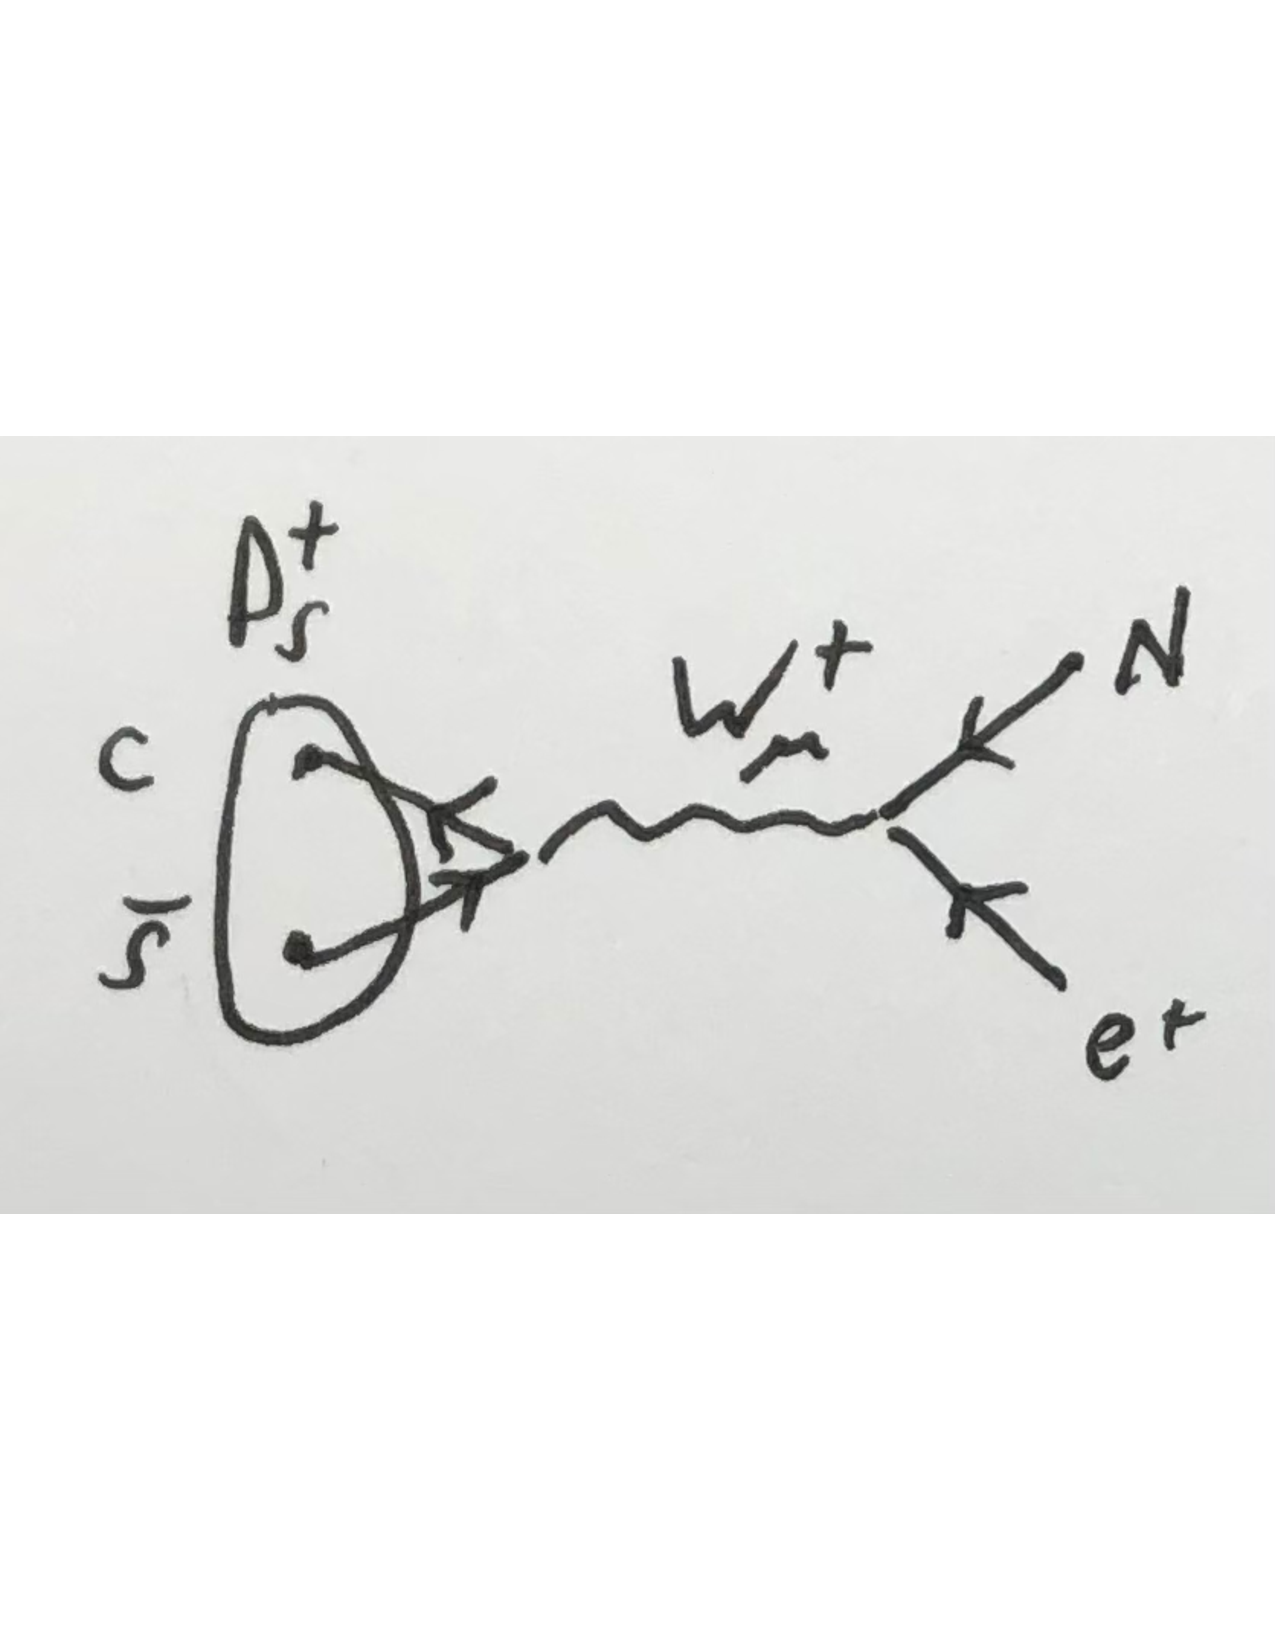
\includegraphics[scale=.18]{meson_decay.pdf}
	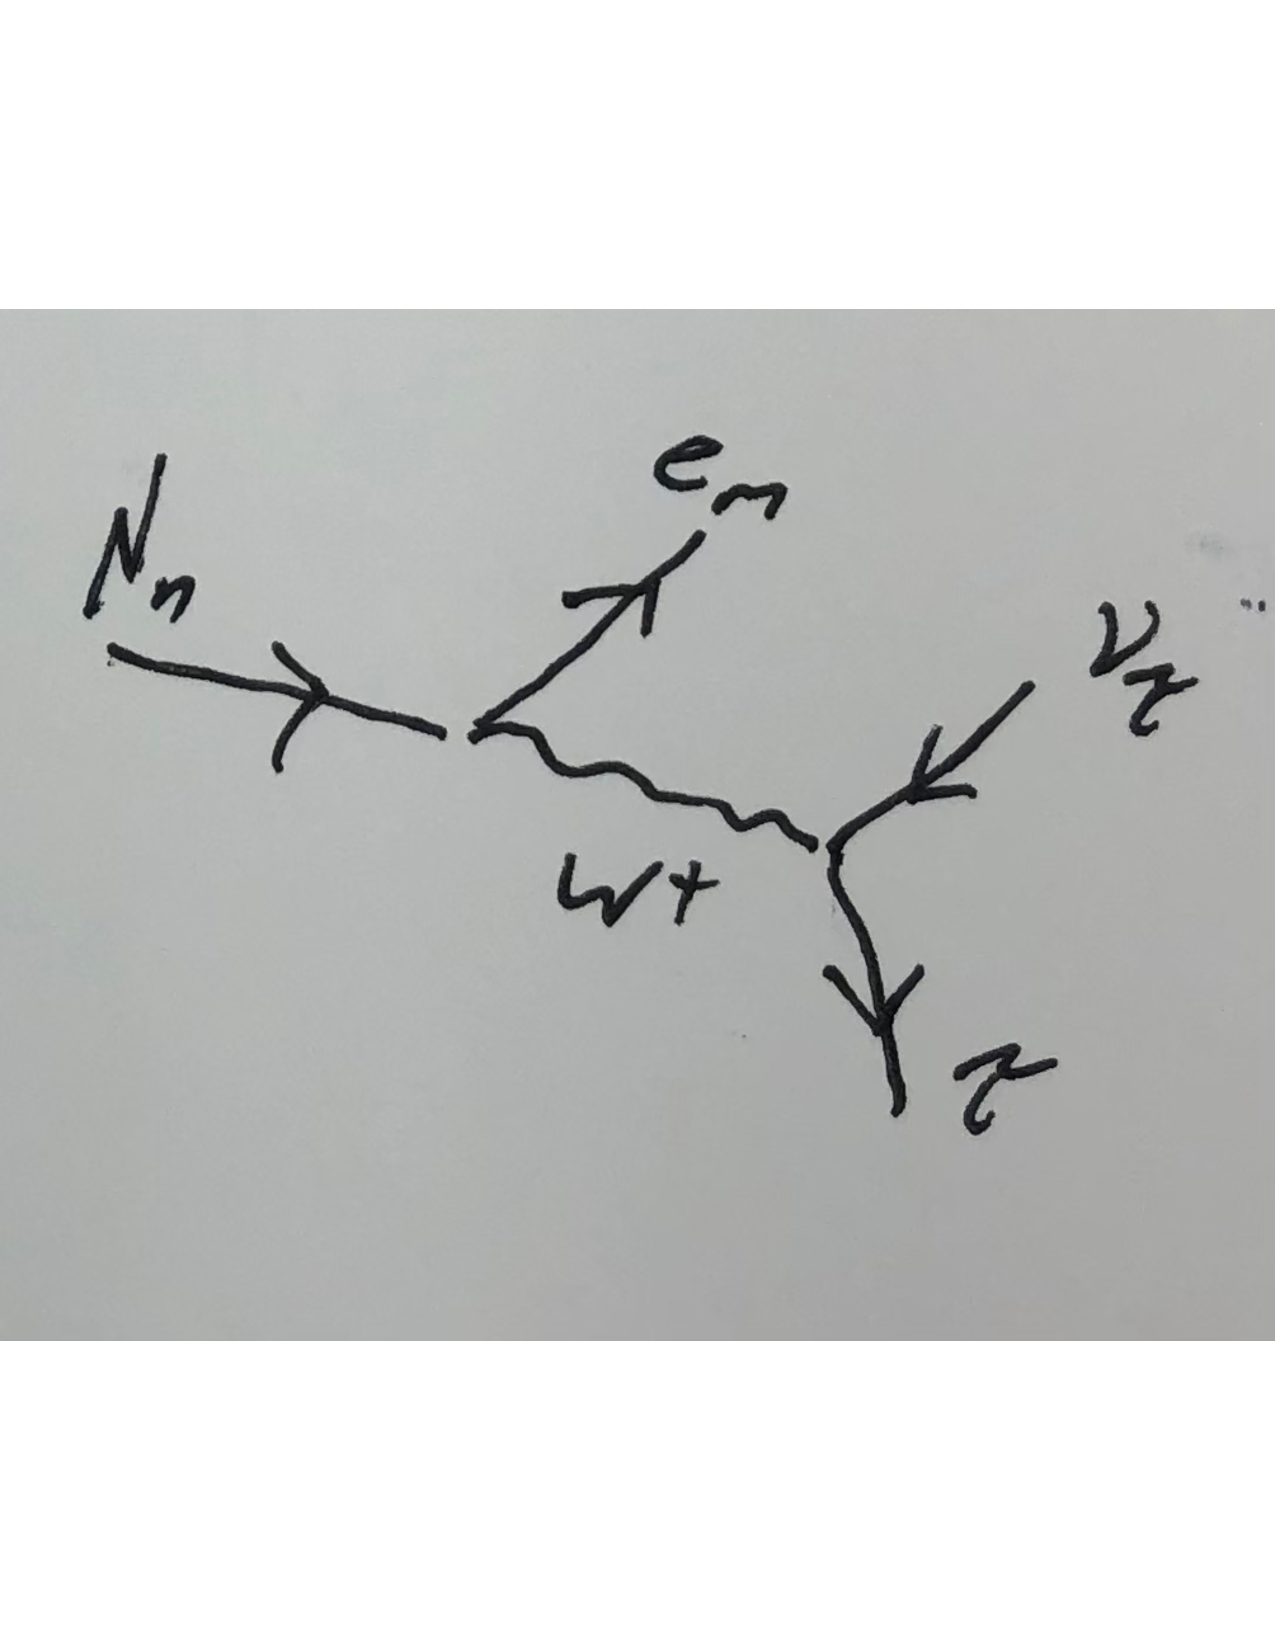
\includegraphics[scale=.18]{Ndecay.pdf}
	\vspace*{-1cm}
	 \hspace*{-0cm}
	\caption{Left: proton collision; middle: meson decay; right: N decay}
	\centering
\end{figure}
\end{frame}


\begin{frame}
\frametitle{FORESEE}
	\begin{itemize}
		\item protons collide and produce a bunch of particles, we care about particles that will produce HNL's
		\item main production comes from $D_s$ mesons
		\item FORESEE utilizes Pythia and other generators to produce the spectra for such particles
			\begin{itemize}
				\item the spectra is needed to keep track of the mesons deflection angle and it's momentum, so that we can find the energy and which mesons make it to the detector.
			\end{itemize}
	\end{itemize}





\end{frame}





\begin{frame}
\frametitle{FORESEE Results; Example}
\begin{figure}
	\vspace*{-1cm}
	 \hspace*{-0cm}
	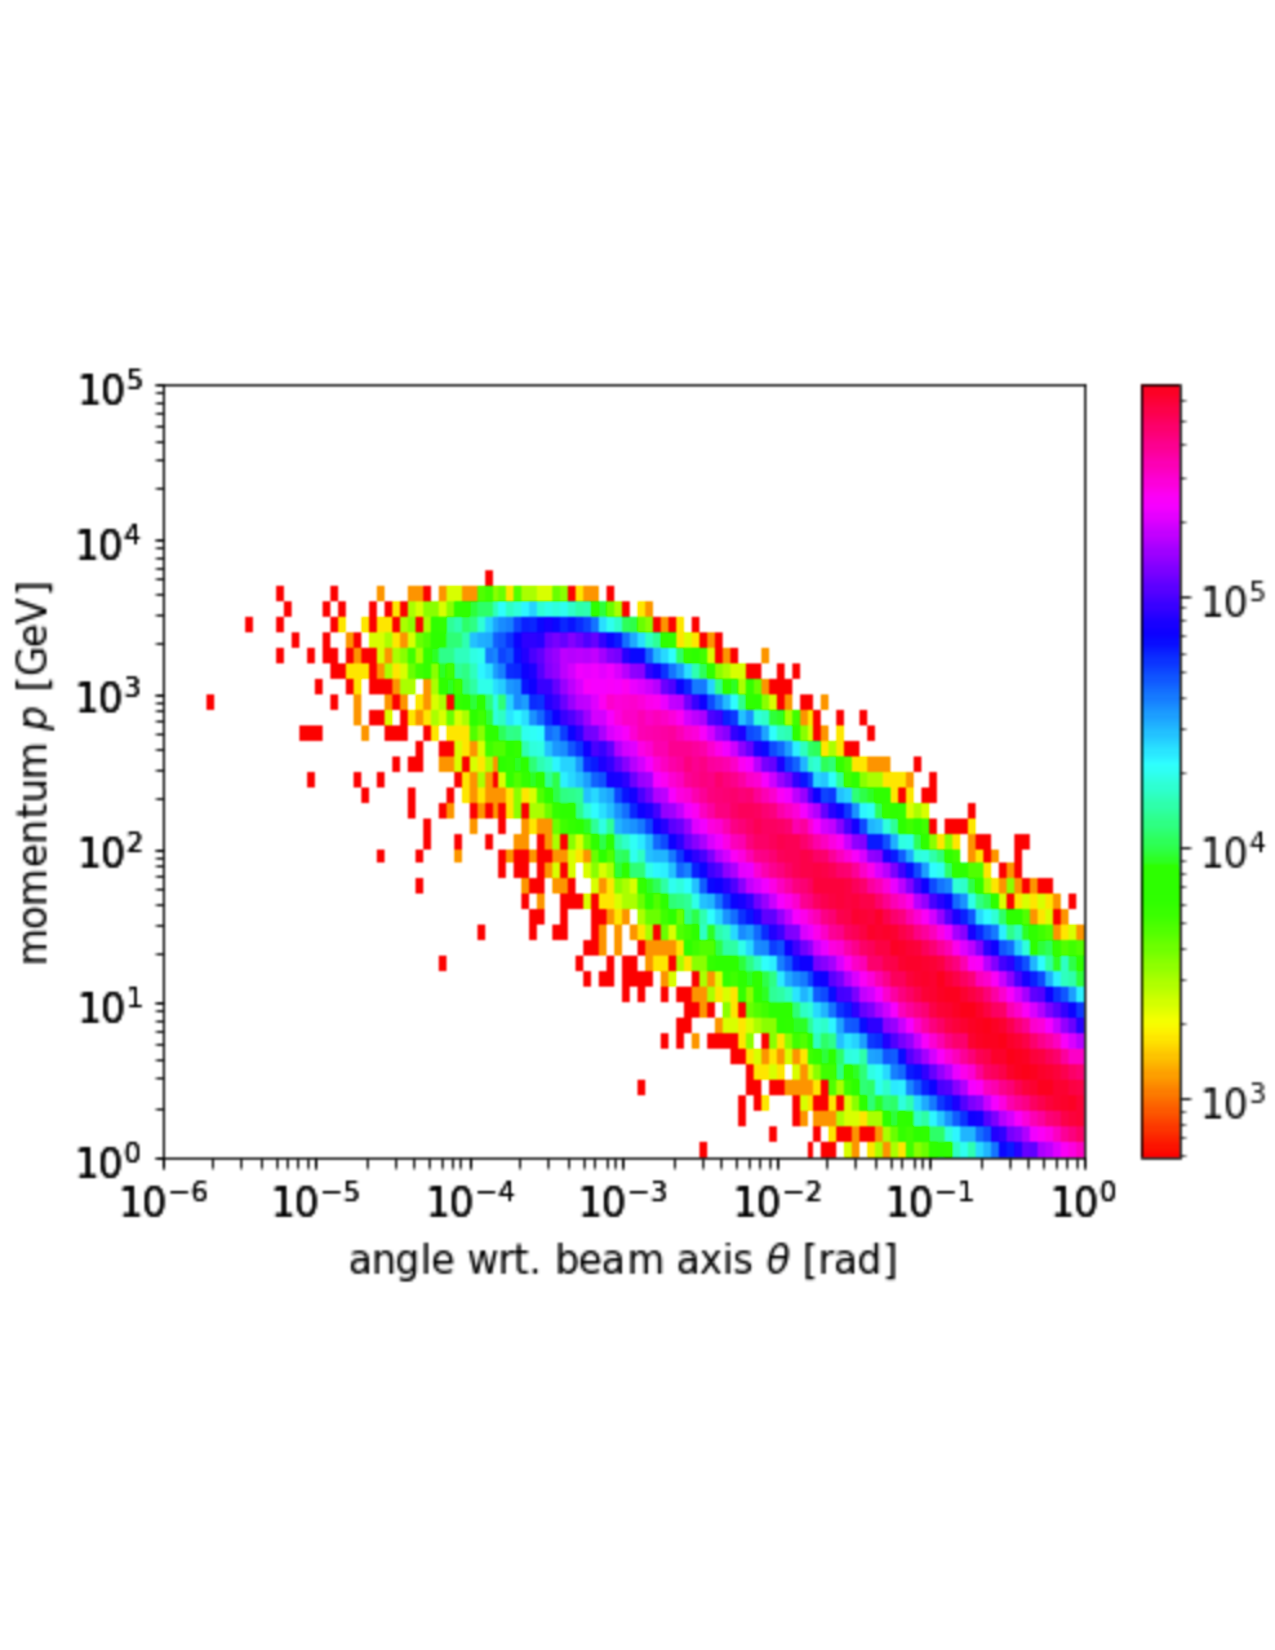
\includegraphics[scale=.18]{Ds_spectra.pdf}
	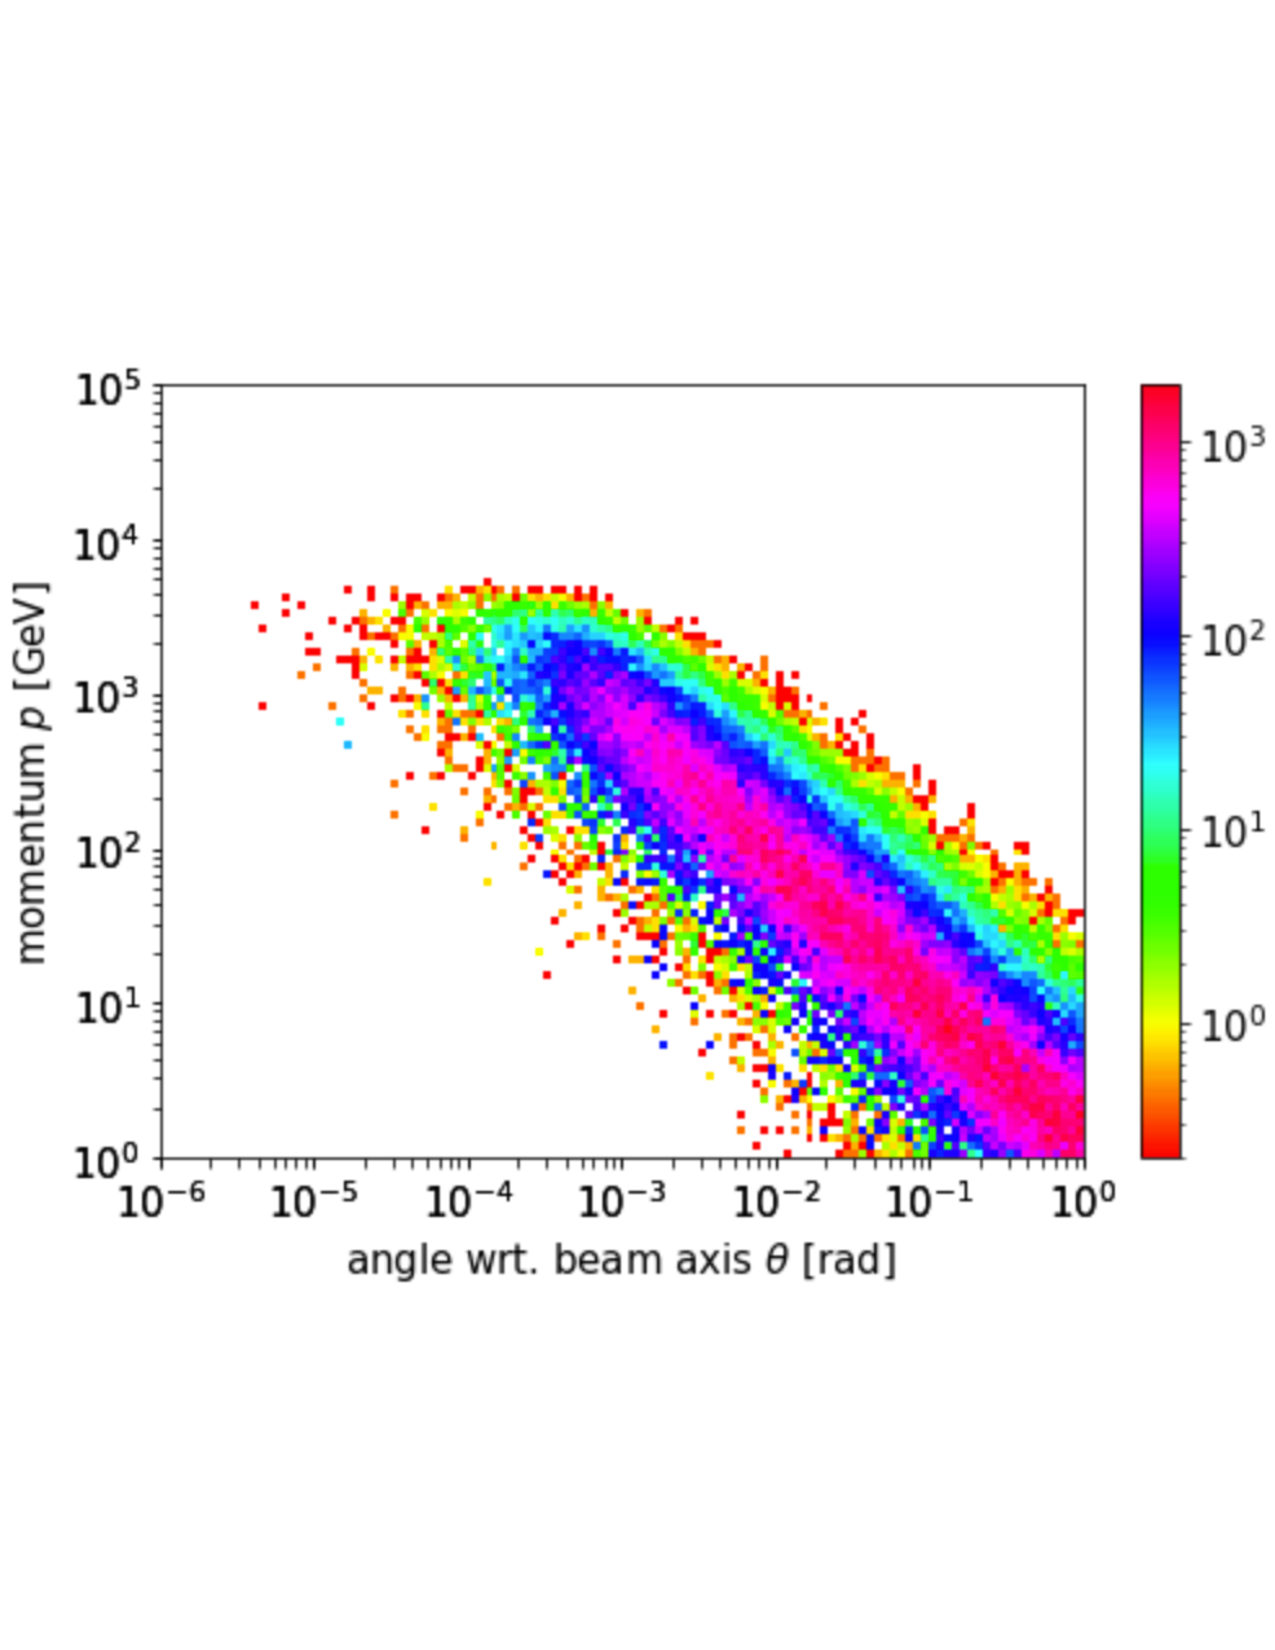
\includegraphics[scale=.18]{HNL_spectra.pdf}
	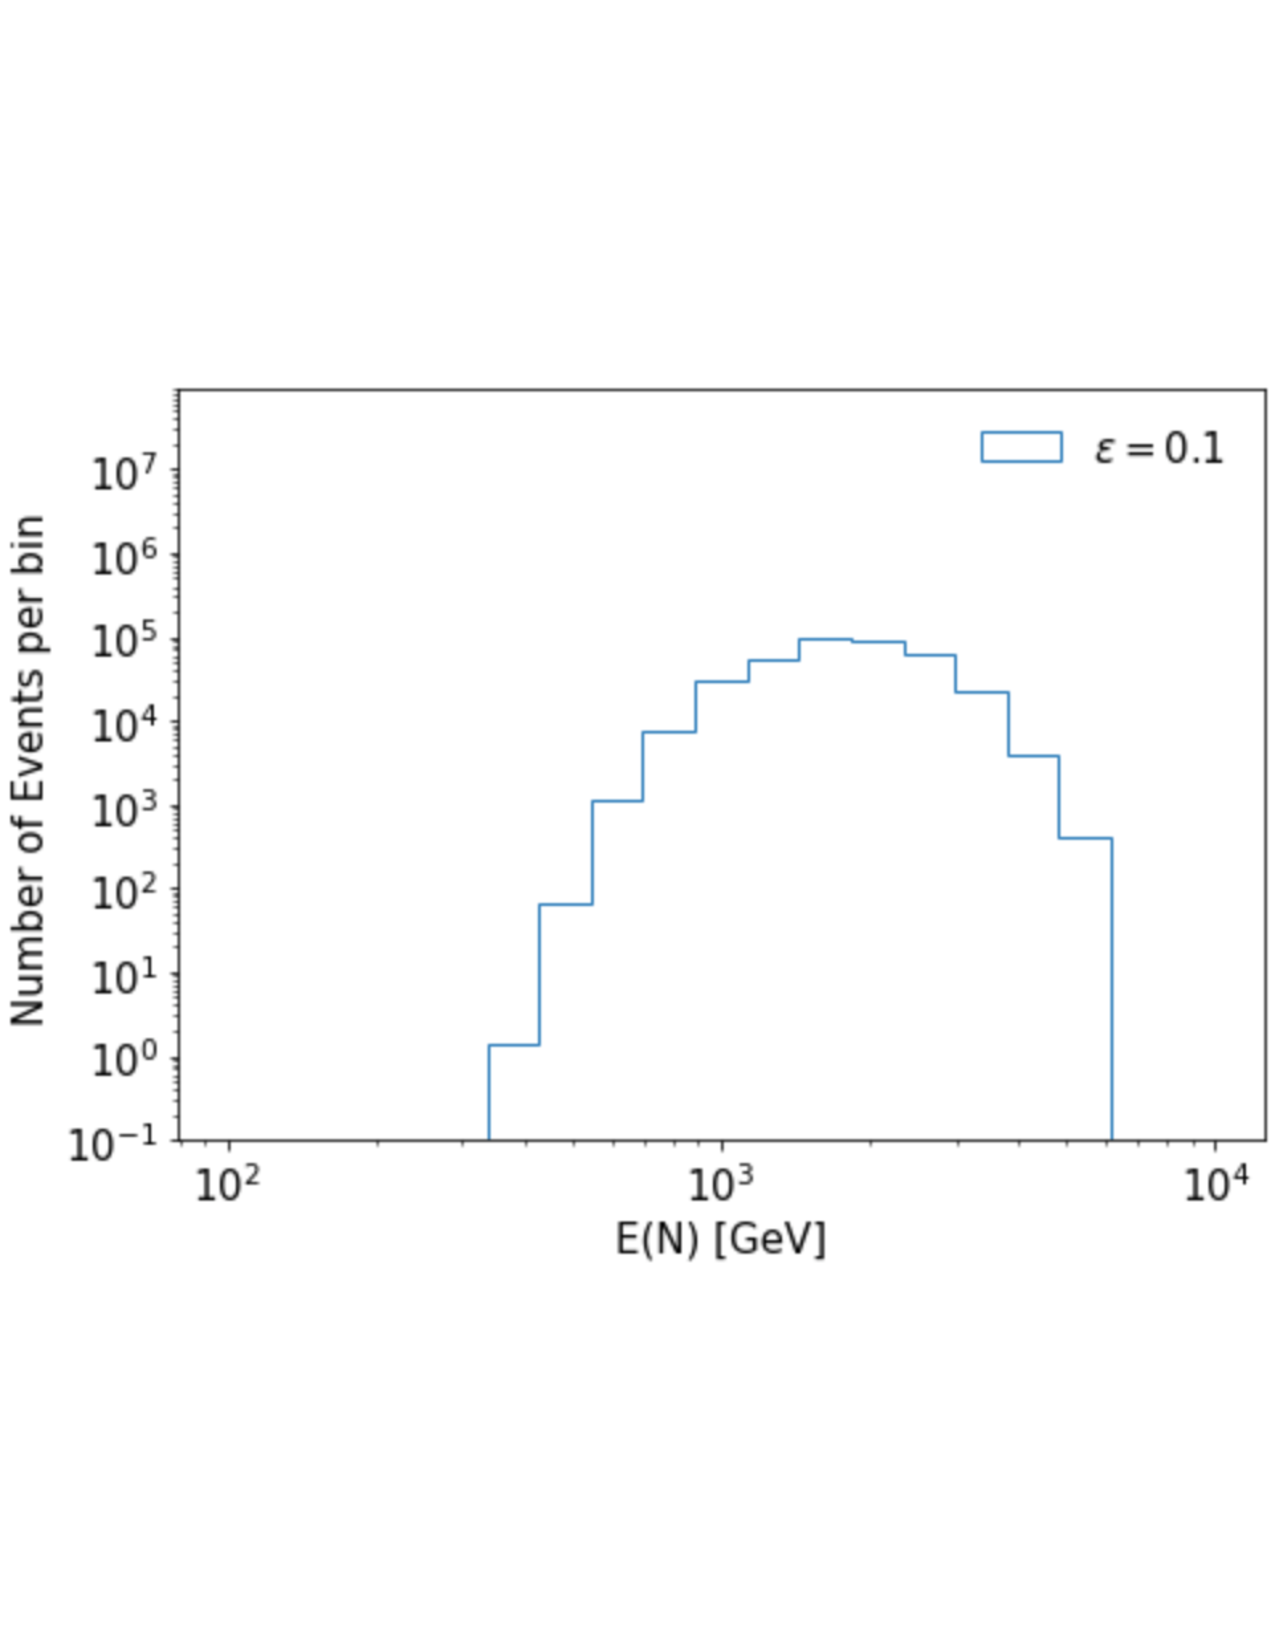
\includegraphics[scale=.18]{NE.pdf}
	\vspace*{-1cm}
	 \hspace*{-0cm}
	\caption{Left: $D_s^+$ spectra, Middle: HNL spectra, Right: E(N) distribution for HNL. $U_e$=.1, $m_{HNL}$=1 GeV; color bar is cross section}
	\centering
\end{figure}
\end{frame}

\begin{frame}
\begin{itemize}
\item to find the number of HNL hits into a certain decay channel we use the formula
\begin{itemize}
\item $n_{sig} = \frac{\sigma_{mother}}{n} \frac{Br(H \rightarrow N + X)}{n} \mathcal{L} \cdot (\text{coupling correction}) \cdot prob_decay \cdot Br(N \rightarrow X)$
\end{itemize}
\end{itemize}
\frametitle{FORESEE Dominant HNL Productions}
\begin{figure}
	\vspace*{-1cm}
	 \hspace*{-0cm}
	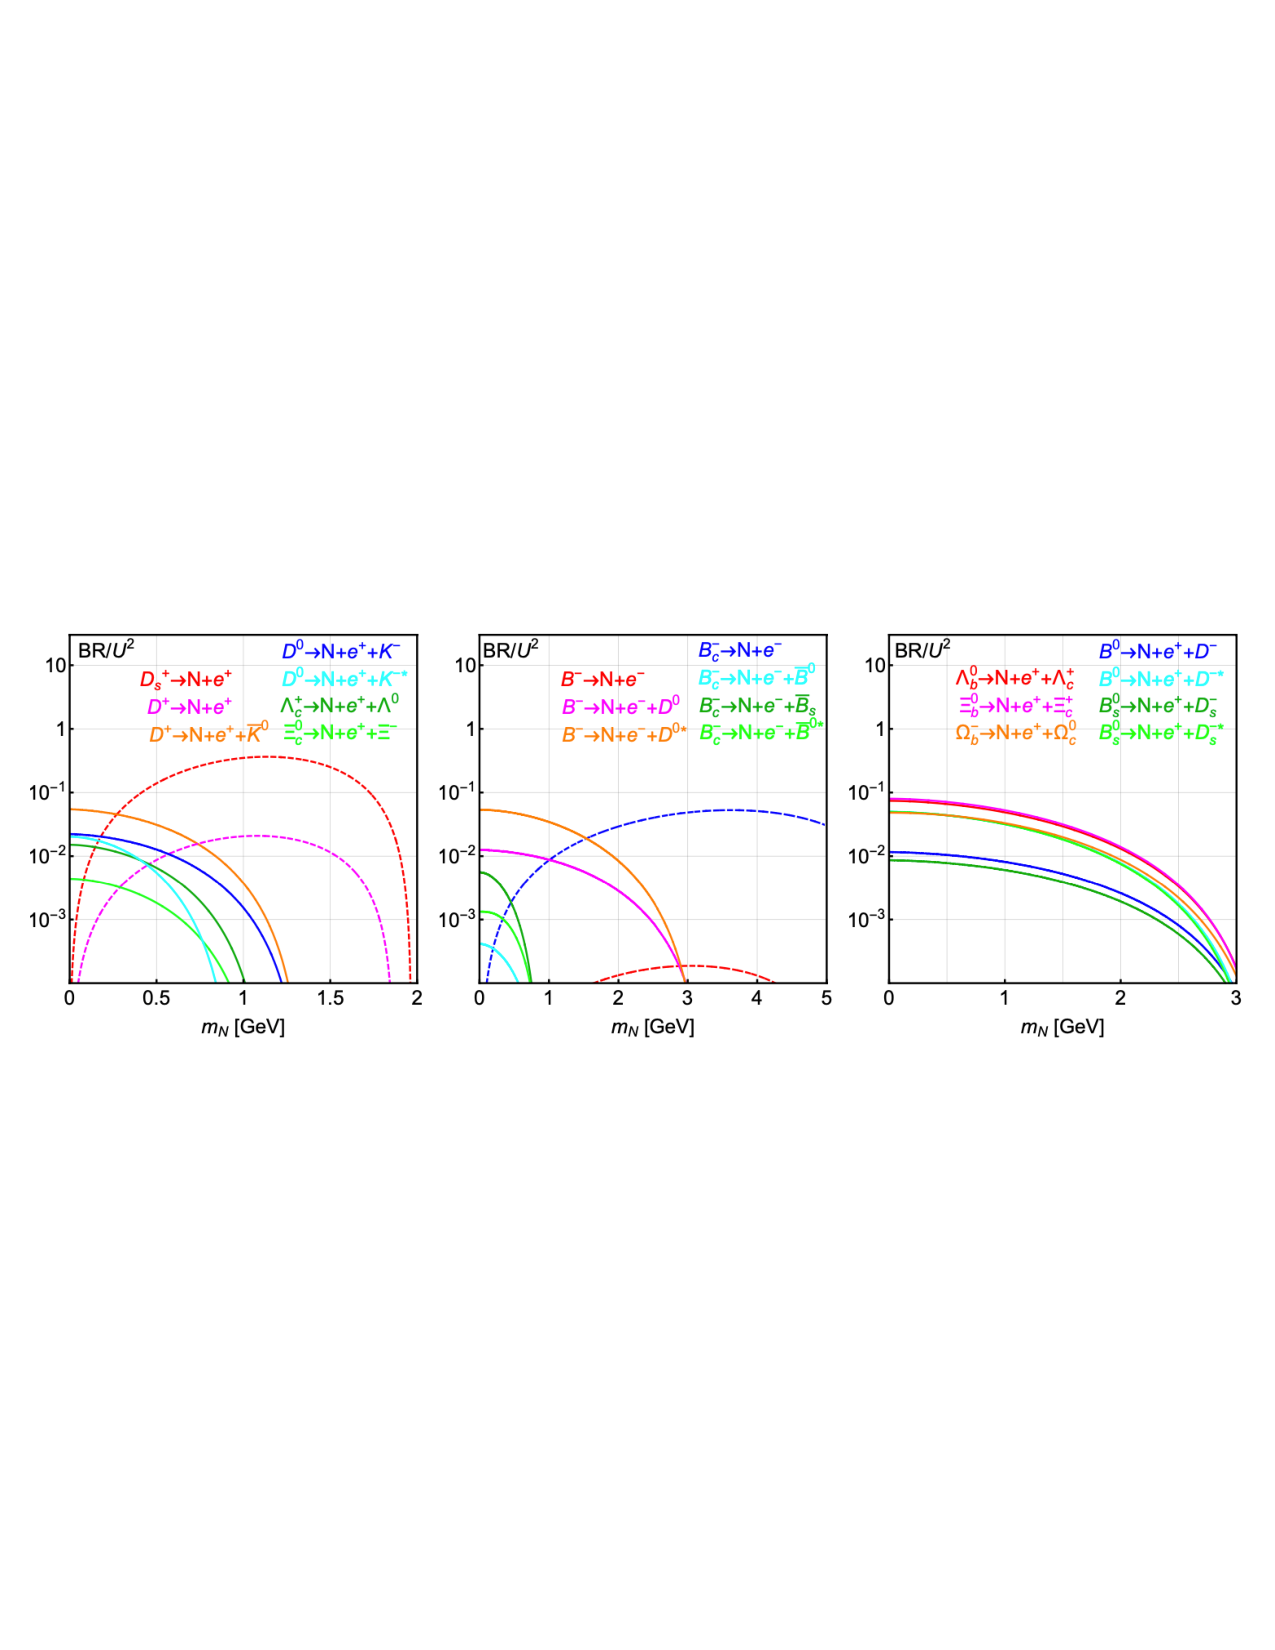
\includegraphics[scale=.4]{Br_dom.pdf}
	\vspace*{-1cm}
	 \hspace*{-0cm}
	\caption{}
	\centering
\end{figure}

\end{frame}


\begin{frame}

\frametitle{Pseudoscalar 2 body decay}
\begin{itemize}
\item Pseudoscalars are mesons with total spin of 0 and odd parity
\end{itemize}
\begin{figure}
	\vspace*{2cm}
	 \hspace*{-0cm}
	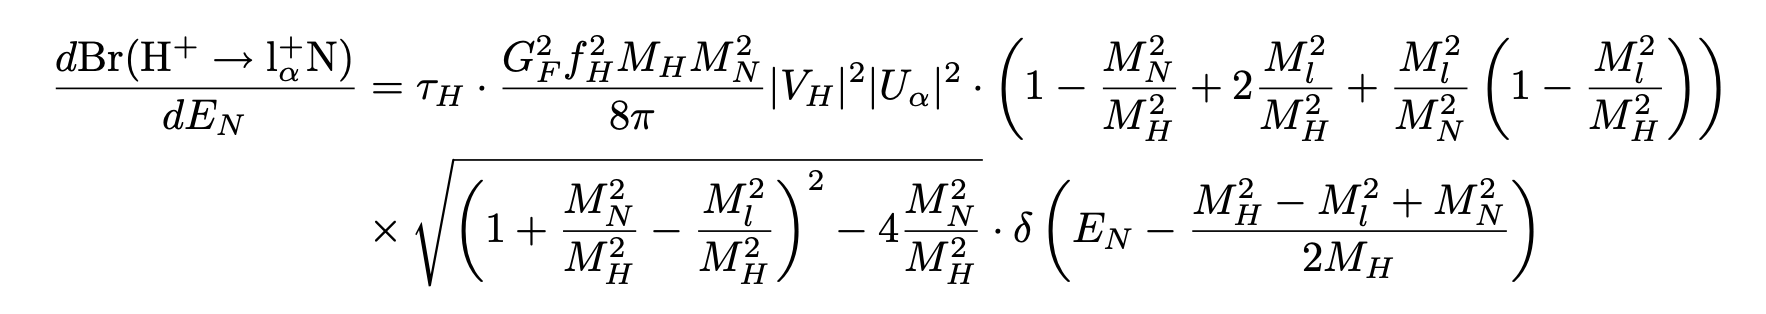
\includegraphics[scale=.4]{2bdy_pseudo}
	\vspace*{-1cm}
	 \hspace*{-0cm}
	\centering
\end{figure}
\end{frame}


\begin{frame}

\frametitle{Pseudoscalar 3-body}

\begin{itemize}
\item these are processes where we begin with a pseudoscalar and end with a pseudoscalar
\item they are more difficult due to form factors and Dalitz plots for 3 body decays
\end{itemize}
\begin{figure}
	\vspace*{0cm}
	 \hspace*{-0cm}
	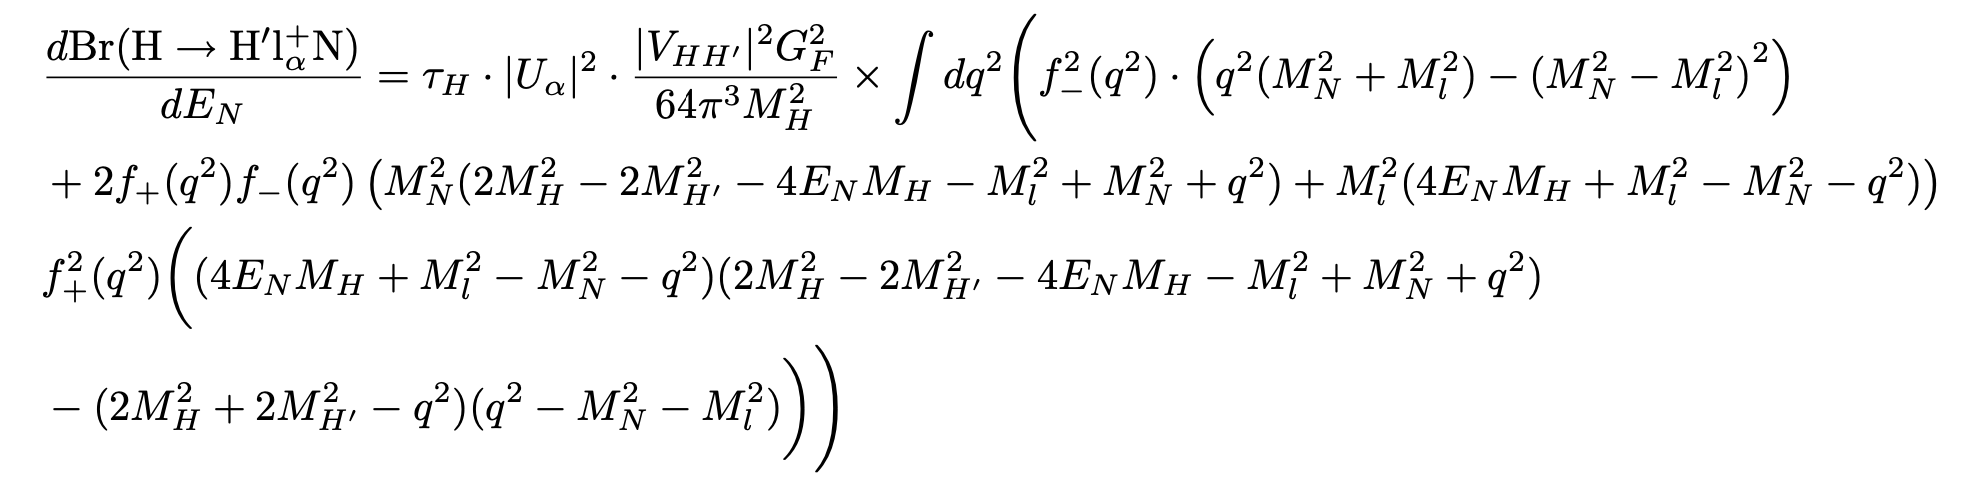
\includegraphics[scale=.4]{pseudo_decay}
	\vspace*{-1cm}
	 \hspace*{-0cm}
	\centering
\end{figure}
\end{frame}

\begin{frame}
\frametitle{Vector 3-body}
\begin{itemize}
\item vector mesons have a total spin of 1 and an odd parity
\end{itemize}

\begin{figure}
	\vspace*{1cm}
	 \hspace*{-0cm}
	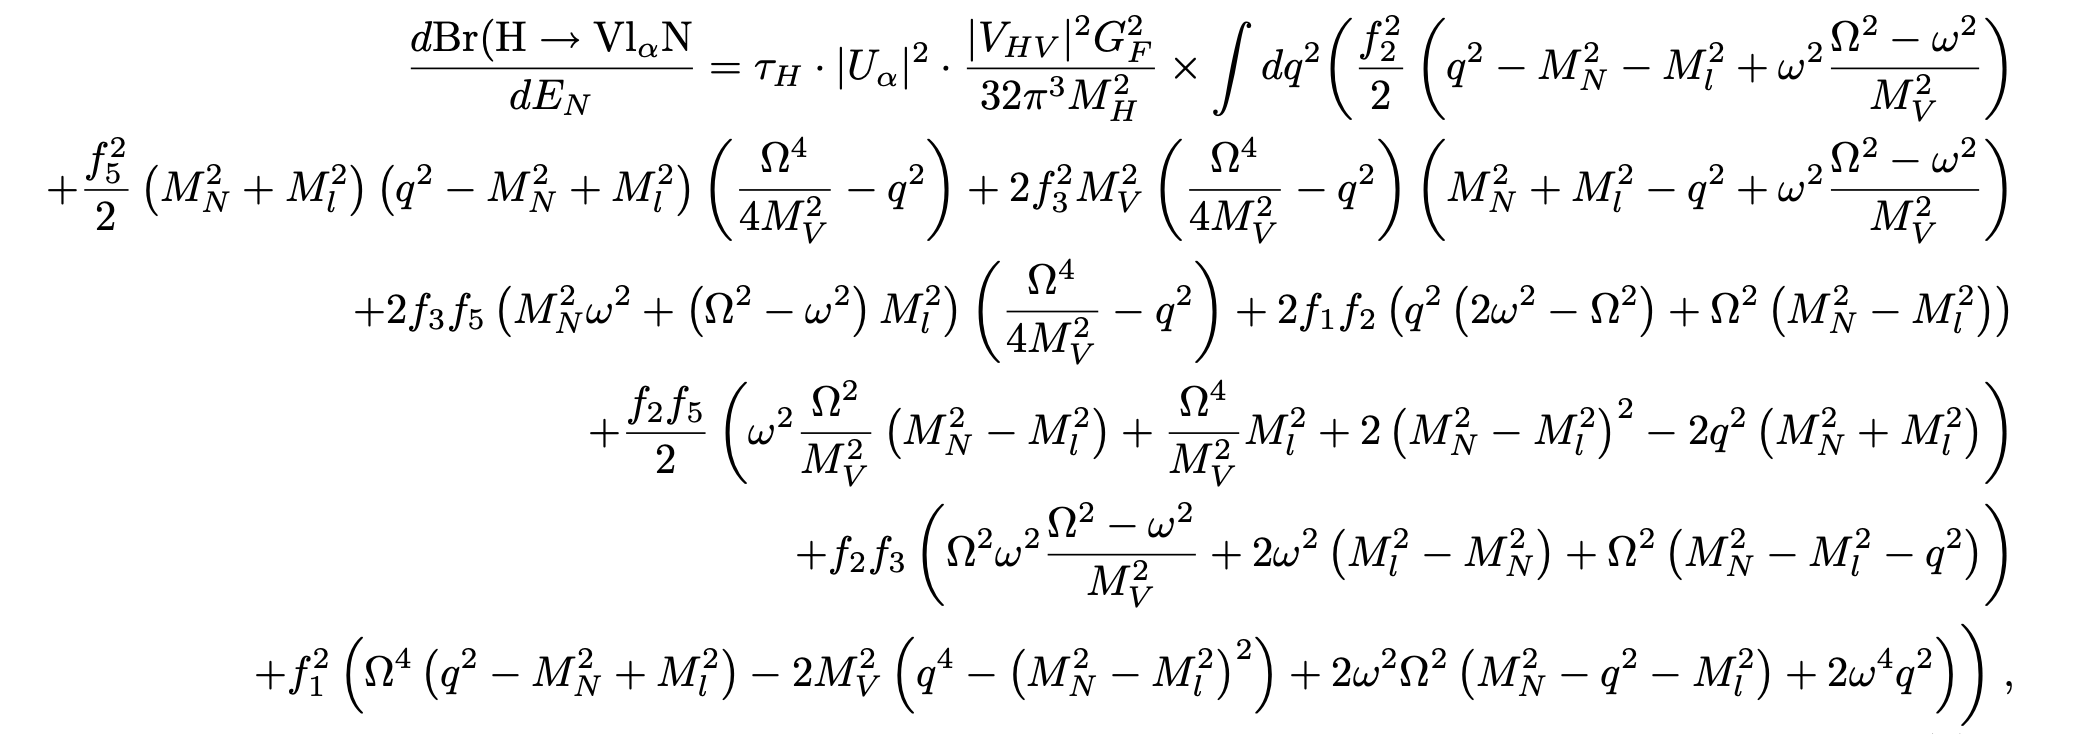
\includegraphics[scale=.4]{pseudo_vec_3bdy}
	\vspace*{-1cm}
	 \hspace*{-0cm}
	\caption{}
	\centering
\end{figure}
\end{frame}

\begin{frame}
\frametitle{Tau Particle Decays}
\begin{figure}
	\vspace*{1cm}
	 \hspace*{-0cm}
	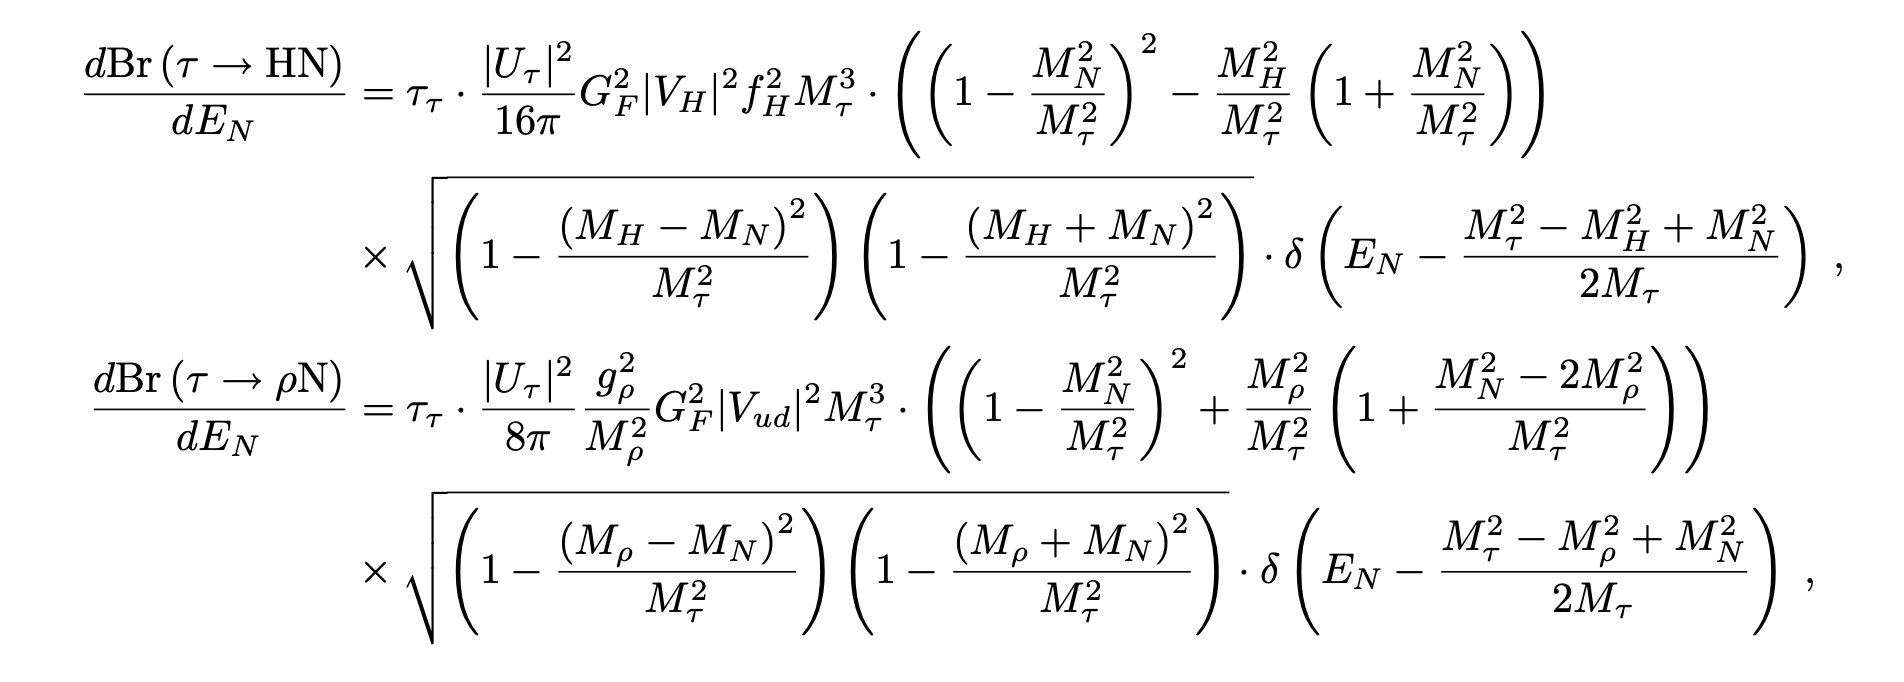
\includegraphics[scale=.3]{tau_2bdy}
	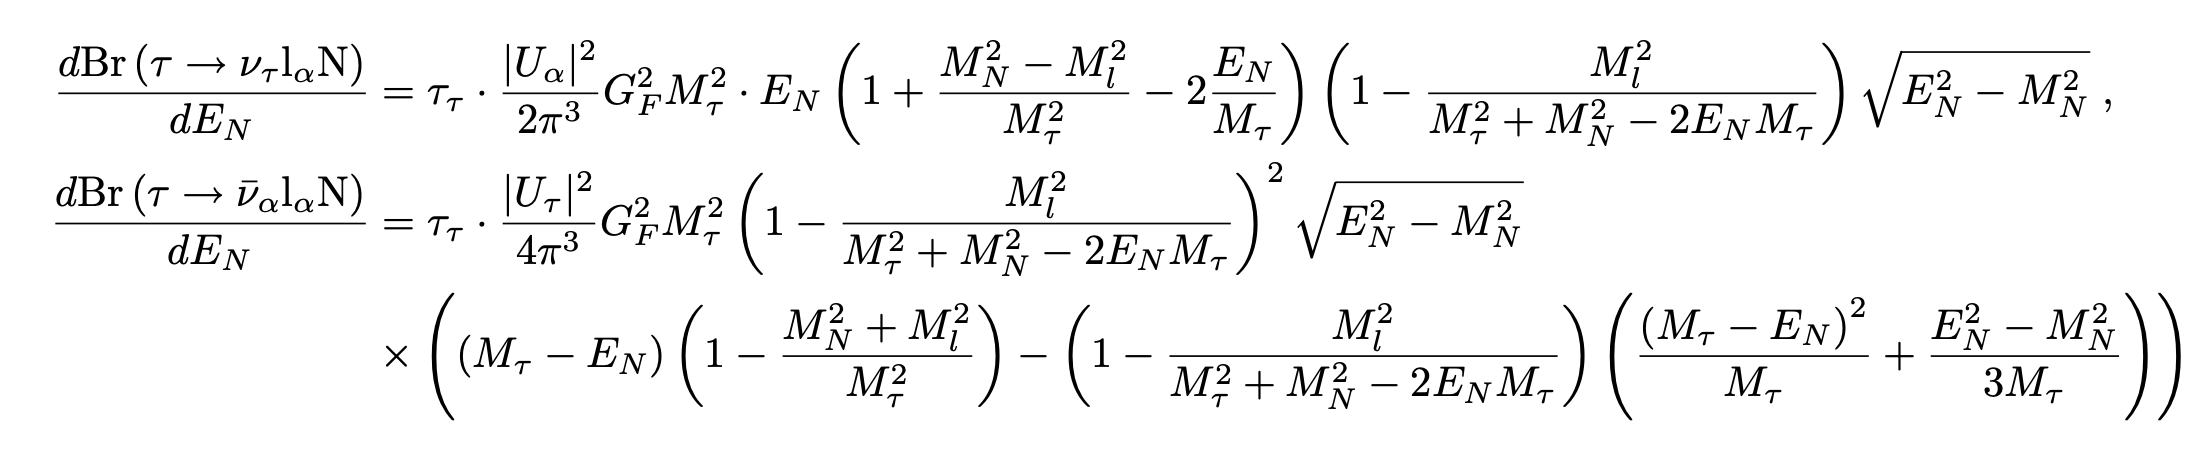
\includegraphics[scale=.3]{tau_3bdy}
	\vspace*{3cm}
	 \hspace*{-0cm}
	\centering
\end{figure}
\end{frame}


\begin{frame}
\frametitle{Whats Next?}
\begin{itemize}
\item next we will include decays into HNL coming from baryons
\item next our focus will shift into the main decay channels for the HNL so we can determine signals for each of the decay channels
\end{itemize}
\begin{figure}
	\vspace*{-2cm}
	 \hspace*{-0cm}
	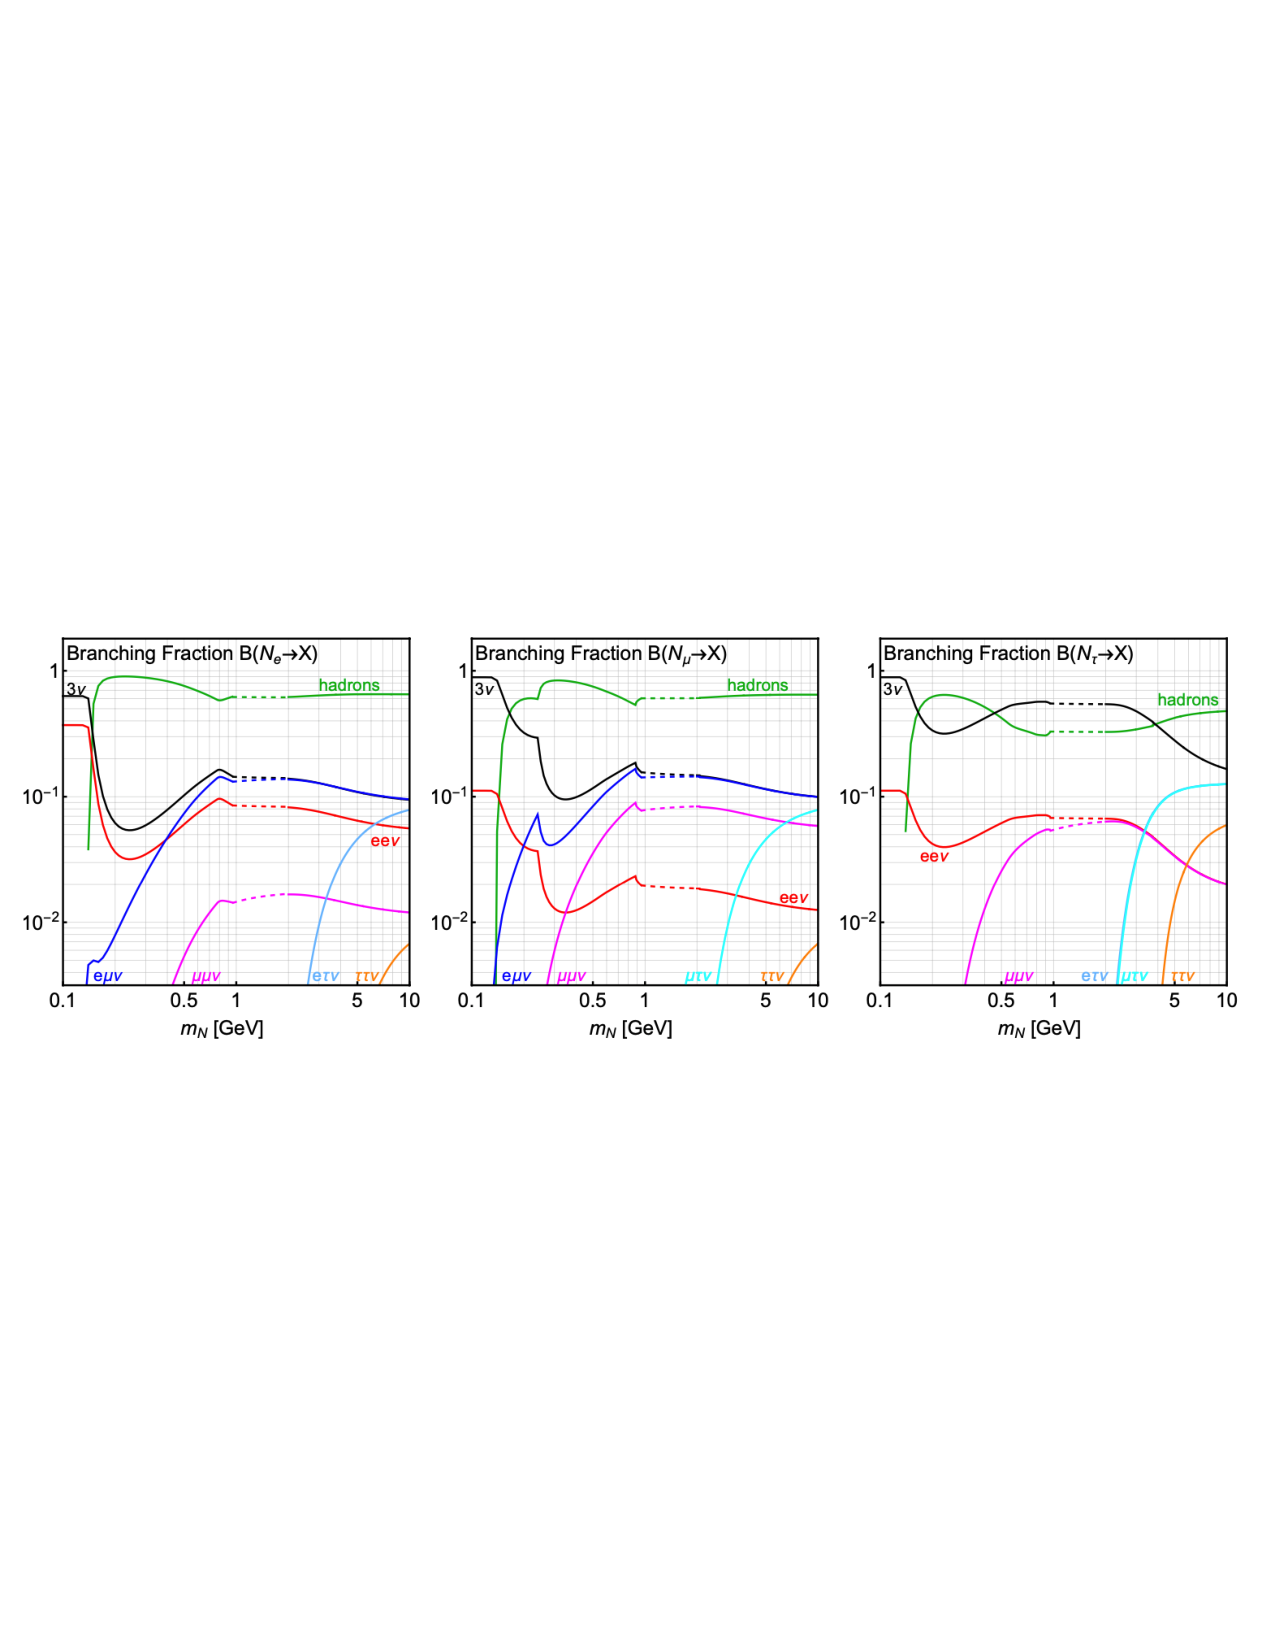
\includegraphics[scale=.4]{had_br_dom}
	\vspace*{-1cm}
	 \hspace*{-0cm}
	\caption{}
	\centering
\end{figure}
\end{frame}









\begin{frame}[plain] % The optional argument 'plain' hides the headline and footline
	\begin{center}
		{\Huge The End}
		
		\bigskip\bigskip % Vertical whitespace
		
		{\LARGE Questions? Comments?}
	\end{center}
\end{frame}



%----------------------------------------------------------------------------------------

\end{document} 